\documentclass[a4paper]{article}
\usepackage{amsmath}
\usepackage{appendix}
\usepackage{amssymb}
\usepackage{algorithm}
\usepackage[noend]{algpseudocode}
\usepackage{tikz}
\usetikzlibrary{shapes.geometric, calc,shapes.multipart,chains,arrows,positioning,automata, trees, fit}
\usepackage{verbatimbox}
\usepackage{textcomp}
\usepackage{pgfplots}
\pgfplotsset{width=10cm,compat=1.9}






\title{Algorithms And Data Structures}
\author{Rory Boyes}
\begin{document}
\maketitle









\titlepage
\tableofcontents
% \begin{abstract}
%   This is my cool abstract using latex for the first time,
%   I will begin to make make my first document. 
%   Though it will take a good deal of time to learn the basics,
%   I am sure it will pay off in the long run. This is a short abstract
%   and should be included after the contents page for formality  to give a
%   brief overview of the contents of the document
% \end{abstract}
\newpage



%========================================================================================%
\section{Project 1}
\subsection{Computational Complexity}

\begin{algorithm}
\caption{Triple Nested For Loop with Variable Assignment and Increment}\label{euclid}
\begin{algorithmic}[1]
\Procedure{ADL for Analysis}{}
\State$for$ $i \leftarrow 1$ to $n$ by $1$ do 
\State\quad $for$ $j \leftarrow 1$ to $i$ by $1$ do 
\State\quad \quad $for$ $k \leftarrow 1$ to $j$ by $1$ do 
\State\quad \quad \quad $x = x +1$
\State\quad \quad $end$
\State\quad $end$
\State$end$ 
\EndProcedure
\end{algorithmic}
\end{algorithm}


\begin{itemize}
  \item Let $f$ represent the body of our function.
  \item Let $n$ represent the input value of our function,
  an integer variable which tends to infinity.
  \item Let $f(n)$ denote the total number of instructions executed when $f$ is applied to $n$.
  \item Let $T$ represent time.
  \item Let $T(n)$ be the relative runtime of our function,(complexity/$T$).$\\
  $T(n) is a numerical value which represents the runtime of a given function
  relative to an arbitrary size of input, from which we can infer it's order of growth.
  \item Let $\theta$ be a tight bound on $T(n)$, which denotes both the asymptotic upper-bound, $(O)$,
  as well as the asymptotic lower bound, $(\omega)$, of a given function, $f$.
\end{itemize}
It is clear from the outset that our space complexity is $O(1)$, as our integer assignments allocate
a constant amount of memory, despite the incrementation of $x$. To contrast, if our inner statement involved the assignment of a new 
variable within a dynamic data structure which was constructed outside of the outer loop, then our
space complexity would become dependant upon $n$.\\\\
We can derive $T(n)$ formally by expressing our function as the following triple summation; \\ 

$$T(n) = \sum_{i=1}^n \sum_{j=1}^i \sum_{k=1}^j c$$\\
Notice that the inner summation index, $k$, is not present within the operation of our innermost summation,
and can therefore be represented as a constant, $c$.\\
\\We can therefore simplify our innermost $k$ summation as following, where $T(n) = $ to the sum from $i=1$ to $n$,
of the sum from $j=1$ to $i$, of the summand..($j$) multiplied by the number of present terms (the top bound$-$ the 
bottom bound )+1, multiplied by our operation constant, $c$.

$$ \therefore T(n) = \sum_{i=1}^n \sum_{j=1}^i(j-1+1)c  $$\

This can be further simplified as following; \\
$$  \sum_{i=1}^n \sum_{j=1}^ijc  $$ \\
To begin resolving our $j$ summation, it must be noted that the index, $j$ is present within the inner operation. 
At this stage, we can either bound the summation, by deriving an upper and lower bound, or by applying a suitable formula. 
In our case, we are dealing with an arithmetic sum, (we are summing $j$), and thereby by factoring out c, we can directly apply
the sum of natural numbers as following; \\
$$ \sum_{i=1}^n i = \dfrac {n(n+1)}{2} $$\\
$$ \therefore T(n) \sum_{i=1}^n \sum_{j=1}^ic = \sum_{i=1}^nc \dfrac{i(i+1)}{2} $$\\ 
We may now arithmetically combine our constants while distributing $i$ resulting in the following summation; \\
$$ T(n) = \sum_{i=1}^n \dfrac {c}{2}(i^2+i) $$\\
By factoring out $\dfrac{c}{2}$, and distributing our summation, we can make use of the following formula, the sum of squares of natural numbers; \\
$$ \sum_{i=1}^n i^2 = \dfrac{n(n+1)(2n+1)}{6} $$ \\
$$ T(n) = \dfrac{c}{2} \left[ \sum_{i=1}^n i^2 + \sum_{i=1}^n i \right] $$ \\
$$ \therefore T(n) = \dfrac{c}{2} \left[ \dfrac{n(n+1)(2n+1)}{6} + \dfrac{n(n+1)}{2} \right] $$\\
We now have a closed form expression, containing only basic operations therefore we can deduce its time complexity. We can see that 
our expression involves the addition of 2 products. Constants aside our first product is the result of the multiplication of 3 $n$ terms, resulting in 
the product $n^3$, whilst our second product is the result of the multiplication of 2 $n$ terms, resulting in the product $2^n$. 
As the addition operator is a linear operator, and we are only interested in the dominant term we can drop the constant factors and low-order terms, therefore
we have determined that $T(n) \in \theta (n^3)$ and is thereby of exponential time complexity, more specifically,
the time complexity is cubic, and therefore also of polynomial time complexity, more broadly speaking.
By tightly bounding our function we have deduced both the upper, and lower bound simultaneously, 
as we may state that the function has a strict runtime, which may only deviate by a value asymptotically less than that of our complexites exponent,  We can therfore 
state that both $O(n)$ and $\omega(n)$ of $f(n)$ are equivalent, and that taking the lower and upper bounds separately would be a provide no further insight. \\



\subsection{Incorporation of Formative Feedback}



\newpage
%========================================================================================%







%========================================================================================%
\section{Project 2}
When devising an algorithm for sorting plates, one must consider not only suitable data structures,
and their effect on time/space complexity, but also the real world implications of sorting these physical
items. We must differentiate between the notion of space, in computing terms, and that of the physical realm.\\

\subsection{Algorithms in ADL}


\begin{algorithm}
\caption{Iterative Quick Sort}\label{euclid}
\begin{algorithmic}[1]
\Procedure{sortStack}{}
\State{\tt (stack: Stack<Integer>,} 
\State{\tt validPlateSizes: HashSet<Integer>)} 
\State{\tt returns Stack<Integer>} \\
\State\quad{\tt sortedStack := create a new Stack<Integer>}
\State\quad{\tt while stack is not empty}
\State\quad\quad{\tt temp := stack.pop()}
\State\quad\quad{\tt if temp is in validPlateSizes}
\State\quad\quad\quad {\tt while sortedStack is not empty}
\State\quad\quad\quad {\tt and sortedStack.peek() < temp}
\State\quad\quad\quad \quad{\tt stack.push(sortedStack.pop())}
\State\quad\quad\quad{\tt end while}
\State\quad\quad\quad{\tt sortedStack.push(temp)}
\State\quad\quad{\tt end if}
\State\quad{\tt end while}
\State\quad{\tt return sortedStack} \\
{\tt end procedure}
\EndProcedure
\end{algorithmic}
\end{algorithm}

The time complexity of the sortStack algorithm above is $O(n^2)$, 
where $n$ is the number of elements in the input stack. 
This is due to the presence of nested loop which iterates over the elements of the stack. 
The inner loop, which is executed once for each element in the stack,
has a time complexity of $O(n)$ as it iterates over all elements in the sorted stack.
The outer loop also has a time complexity of $O(n)$ because it iterates over all elements in the input stack.
Therefore, our overall time complexity is $O(n^2)$.\\

The space complexity of the algorithm is $O(n)$, as the algorithm uses a single stack to store the sorted elements.
The size of the stack grows linearly with the number of elements in the input stack, so the space complexity is $O(n)$. \\


If space complexity was our primary concern, this approach would acceptable.
Utilizing a hashed set for checking our valid plate sizes will prevent us from traversing during this operation, 
but despite this, our function is still $O(n^2)$, as the fastest growing term takes precedant. \pagebreak



% To improve the time complexity of our solution. we can create a number of stacks equal to the number of valid values, 
% or in our case, valid plate sizes. By avodiding comparioson operations, and traversal, we can reduce the possible number of 
% forks of the upper bound to n, resulting in linear time complexity. By utiziling hashing we can avoid traversal, and
% reduce our \\

% We can improve this approach further by representing each stack of plates as a single value, which we can then 
% increment upon addition, and decrement upon removal. As we previously allocated $n$ node spaces 
% in the form of a linked list for each key value pair of our map, allowing for the entire reversal of the 
% intial stack, this imroved implementation will drastically reduce our additional space complexity, from $n^3 +n$
% to simply $n+n = n$ \\



\begin{algorithm}
\caption{Bucket Method with Hashing}\label{euclid}
\begin{algorithmic}[1]
\Procedure{sortStackWithMap}{}
\State{\tt (map: Hashmap<Integer, Integer>,}
\State{\tt stack: Stack<Integer>)} \\

\State\quad{\tt popped: Integer}
\State\quad{\tt while stack is not empty}
\State\quad\quad{\tt popped <- stack.pop()}
\State\quad\quad{\tt if map contains key popped}
\State\quad\quad\quad{\tt map.put(popped, map.get(popped)+1)}
\State\quad\quad{\tt end if}
\State\quad{\tt end while}\\

\State\quad{\tt for(each key in map)}
\State\quad\quad{\tt while key > 0}
\State\quad\quad\quad{\tt stack.push(key)}
\State\quad\quad\quad{\tt map.put(key, map.get(key)-1)}
\State\quad\quad{\tt end while}
\State\quad{\tt end for} \\
{\tt end procedure}
\EndProcedure
\end{algorithmic}
\end{algorithm}




The time complexity of the algorithm above is $O(n)$,
where $n$ is the number of elements in the input stack. 
This is because the algorithm performs a single pass over the elements of the stack,
counting the number of occurrences of each element inside of the hashmap. 
The time complexity of this operation is $O(n)$, 
as the hash map has an average-case time complexity of $O(1)$ for insertion and retrieval of elements
due to usage of a hashing function.
$\therefore$ the $T(n)$ grows linearlly with the size of the input. \\

It is worth noting that if we were to use another data type such as a string to represent each plate type,
a linked list value store impentation of a hash map could decay to $O(n^2)$ in the worst case, due to collisions.
As we are using integers we may also state that  $T(n) \in \theta (n)$ \\

The space complexity of the function is also $O(n)$,
as the hashmap used to store the counts of each element of the unsorted stack
grows linearly with the number of elements in the input stack,
ie, there is no possibility that the number of elements within the hashmap could ever exceed that of the input stack.
$\therefore$ the space complexity is $O(n)$. \\

Furthermore, had we not been working under the constaint of only moving one element at any given time,
the time complexity of the algorithm could be improved further
to $O(n log n)$ by sorting the elements in the hashmap before pushing them back onto the stack.
However, this would be at the detriment of additional space complexity,
as the usage of a sorting algorithm, such as quick or merge sort, 
would require additional space to store auxiliary structures such as partition indices. \\ 

% It so happens that have no requirment to sort due to the value of our map being used purely as 
% a means to increment a value which represents the number of plates of said size, or type, our key.
% Therefore in a less general sense, we could quanitify that given our specific parameters,
% $T(n) = O(n log n)$. \\


\subsection{Data Structures} 
\vspace{4mm}


\makeatletter
\renewcommand{\ALG@name}{Structure}
\makeatother
\setcounter{algorithm}{0}

\begin{algorithm}
\caption{HashMap}\label{euclid}
\begin{algorithmic}[1]



\algrenewcommand\algorithmicprocedure{\textbf{public class}}
\Procedure{HashMap}{\tt <K, V>} {\{} \\
\State{\tt private static final int DEFAULT\_CAPACITY = 16;}
\State{\tt private static final double LOAD\_FACTOR = 0.75;}
\State{\tt private int capacity;}
\State{\tt private int size;}
\State{\tt Entry<K, V>[] bucket;}
\EndProcedure
\end{algorithmic}
\end{algorithm}

A bucket is a term used to describe a space in the array that stores entries of the same hash code.
Capacity determines how many buckets are available in the hash map, and therefore,
how many Entry objects can be stored in the map before the map needs to be resized. \\

The default capacity constant field determines the initial size of the array
used to store entries, (key value pairs). 16 has been chosen as a sane default,
as it is a power of 2, and $\therefore$ allows for efficient index calculations using bit shifting,
The default size is small enough to minimize memory overhead,
while large enough to prevent resizing too often.
The initial capacity can also be specified within the constructor, 
by passing the capacity as an argument. 
This could be useful in cases where it is known in advance that the hashmap will need 
to store a large data set, though a larger initial capacity will require more memory. \\


The load factor of a HashMap is the ratio of the number of entries in the hash map to the capacity of the hash map,
and is calculated by dividing the number of entries in the map by the capacity of the map
It is used to determine when the capacity of the hash map should be increased to maintain good performance.
The default maxiumum load factor is defined to allow for the aforementioned resizing once it has been exceeded.
A load factor too high could cause the hashmap to perform poorly as collisions may occur causing our time complexity to decay. 
Contrarily, too low of a load factor is inefficient in regards to space complexity as the resizing will occur prematurely,
resulting in unnecessarily memory allocation. \\

0.75 is a fairly typical load factor for hashmap implementations as it provides a middleground between
these trade offs. The load factor can also be specified by passing a second argument to the constructor upon initializtion. \pagebreak




\makeatletter
\renewcommand{\ALG@name}{Nested Class}
\makeatother
\setcounter{algorithm}{0}

\begin{algorithm}
\caption{Entry}\label{euclid}
\begin{algorithmic}[1]



\algrenewcommand\algorithmicprocedure{\textbf{private static class}}
\Procedure{Entry}{\tt <K, V>} {\{} \\
\State{k key}
\State{v value}
\State{Entry<K, V> next} \\

\State{Entry(K key, V value, Entry<K, V> next) \{ }
\State\quad{this.key = key;}
\State\quad{this.value = value;}
\State\quad{this.next = next;}
\State{\{} \\
\{
\EndProcedure
\end{algorithmic}
\end{algorithm}




The Entry class is a nested class within the HashMap class that represents a key-value pair in the map.
Each Entry has a key and a value, as well as a reference to the next Entry in the bucket of entries,
forming a linked list of Entries within each bucket.
The constructor takes all three of these fields as arguments. \\

The key of each entry is passed through a hash function to determine which bucket it is to be stored in.
If the bucket is empty, the new entry becomes the first entry in the bucket.
If a collision occurs, the new entry is added to the end of the list within the corresponsing bucket.
Subsequently the hash function can again be used to determine which bucket to search 
to retrive the desired key value pair based on the hash of the key.







%================================================%
\vspace{4mm}
\makeatletter
\renewcommand{\ALG@name}{Hashmap Constructor}
\makeatother
\setcounter{algorithm}{0}

\begin{algorithm}
\caption{}\label{euclid}
\begin{algorithmic}[1]

\algrenewcommand\algorithmicprocedure{\textbf{public HashMap}}
\Procedure{HashMap}{} {\{}
\State{\tt this(DEFAULT\_CAPACITY);} \\
{\}}
\EndProcedure
\end{algorithmic}
\end{algorithm}

The default hashmap constructor is the most commonly used,and utliziles the aformented 
predetemined capacity to instatiate a new hashmap with no given arguments.
%================================================%



%================================================%
\vspace{4mm}
\makeatletter
\renewcommand{\ALG@name}{Hashmap Constructor}
\makeatother

\begin{algorithm}
\caption{}\label{euclid}
\begin{algorithmic}[1]

\algrenewcommand\algorithmicprocedure{\textbf{public HashMap}}
\Procedure{HashMap}{int capacity} {\{}
\State{\tt this.capacity = capacity;} 
\State{\tt this.bucket = new Entry[capacity];} \\
{\}}
\EndProcedure
\end{algorithmic}
\end{algorithm}

As mention the second constructor allows specification of initial capacity of the map upon instantiation.
A new array of type Entry is also declared with the specified capacity assigned to the bucket field. \pagebreak






%     \begin{tikzpicture}[%scale=.2,
% node distance = 7mm and 4mm,
%   start chain = going right, 
%    arr/.style = {semithick, -Stealth},
%    dot/.style = {circle, fill, inner sep=1.2pt,
%                  label=left:#1},
% every label/.append style = {font=\footnotesize, fill=white, align=center,
%                              fill opacity=0.5, text opacity=1, 
%                              inner sep=1pt},
%      E/.style = {ellipse, draw, fill=#1},
%   mpnh/.style = {rectangle split, rectangle split horizontal, 
%                  rectangle split parts=3, draw, fill=gray!20,
%                  inner sep=2pt,
%                  on chain},
%   mpnv/.style = {rectangle split, rectangle split parts=10,
%      rectangle split part fill={gray!30,gray!10,gray!30,gray!30,gray!30,
%                                 gray!10,gray!30,gray!10,gray!10,gray!30},
%      draw, minimum height=2ex},
%    sym/.style = {yshift=-1mm},
%    syp/.style = {yshift=+1mm},
%                         ]
% \node[mpnv, label=H] (H) 
%     {\nodepart{one}     $\diagup$
%      \nodepart{two}     \vphantom{$\diagup$} 
%      \nodepart{three}   $\diagup$
%      \nodepart{four}    $\diagup$
%      \nodepart{five}    $\diagup$
%      \nodepart{six}     \vphantom{$\diagup$} 
%      \nodepart{seven}   $\diagup$
%      \nodepart{eight}   \vphantom{$\diagup$} 
%      \nodepart{nine}    \vphantom{$\diagup$} 
%      \nodepart{ten}     $\diagup$
%     };
% %
% \node[mpnh, right=of H.two east] (A1) 
%    {\nodepart{one}  $\diagup$
%     \nodepart{two}  $k_1$
%     \nodepart{three}    \hphantom{$\diagup$}  
%    };
% \node[mpnh] (A2)
%    {\nodepart{one}      \hphantom{$\diagup$}
%     \nodepart{two}      $k_4$
%     \nodepart{three}    $\diagup$
%    };
% %
% \node[mpnh, right=of H.six east] (B1)
%    {\nodepart{one}      $\diagup$
%     \nodepart{two}      $k_5$
%     \nodepart{three}    \hphantom{$\diagup$}
%    };
% \node[mpnh] (B2)
%    {\nodepart{one}      \hphantom{$\diagup$}
%     \nodepart{two}      $k_2$
%     \nodepart{three}    \hphantom{$\diagup$}
%    };
% \node[mpnh] (B3)
%    {\nodepart{one}      \hphantom{$\diagup$}
%     \nodepart{two}      $k_7$
%     \nodepart{three}    $\diagup$ 
%    };
% %
% \node[mpnh, right=of H.eight east] (C1)
%    {\nodepart{one}      $\diagup$
%     \nodepart{two}      $k_3$
%     \nodepart{three}    $\diagup$
%    };
% %
% \node[mpnh, right=of H.nine east] (D1)
%    {\nodepart{one}  $\diagup$
%     \nodepart{two}  $k_8$
%     \nodepart{three}    \hphantom{$\diagup$}
%    };
% \node[mpnh] (D2)
%    {\nodepart{one}      \hphantom{$\diagup$}
%     \nodepart{two}      $k_6$
%     \nodepart{three}    $\diagup$
%    };
% %% arrows (right)
% \draw[arr]  (H |- H.two east)   edge (A1)
%             (H |- H.six east)   edge (B1)
%             (H |- H.eight east) edge (C1)
%             (H |- H.nine east)   to (D1)
%             ;
% \draw[arr, transform canvas={yshift=1mm}]  
%             (A1.three north |- A1.east)  edge (A2)
%             (B1.three north |- B1.east)  edge (B2)
%             (B2.three north |- B2.east)  edge (B3)
%             (D1.three north |- D2)   to   (D2)
%             ;
% \draw[arr, transform canvas={yshift=-1mm}]
%             (A2.one north |- A2)  edge  (A1)
%             (B2.one north |- B2)  edge  (B1)
%             (B3.one north |- B3)  edge  (B2)
%             (D2.one north |- D2)   to   (D1)
%             ;
% %% dots, ellipses
% \pgfmathsetseed{3}
% Explicitly sets the seed for
% \foreach \i in {1,2,...,8}
%     \node (k\i) [dot=$k_{\i}$] at (-33mm +40*rand,0.5*rand) {};


% \scoped[on background layer]
% {
% \draw[fill=gray!30]  (-4,0.4) ellipse (3 and 2);
% \path   (-4,1) node[label={$U$\\ (universe of keys)}] {};

% \draw[fill=white]   (-4,0) ellipse (2.4 and 1);
% \path   (-6,0) node[label=right:$K$\\ (actual\\ keys)] {};

% \draw[arr]  (k1)    edge ([syp] H.two west)
%             (k4)    edge ([sym] H.two west)

%             (k2)    edge ([syp] H.six west)
%             (k5)    edge (H.six west)
%             (k7)    edge ([sym] H.six west)
%             
%             (k3)    edge (H.eight west)
%             
%             (k8)    edge ([syp] H.nine west)
%             (k6)    edge ([sym] H.nine west)
%             ;
% }
%     \end{tikzpicture}




\pagebreak
%================================================%




\pagebreak
\subsection{Software and its Presentation, including testing (and video link)}


\subsection{Descriptive Report, including artefacts}

%===================Hashmap Put Method=======================%

\vspace{4mm}
\makeatletter
\renewcommand{\ALG@name}{Hashmap Method}
\makeatother
\setcounter{algorithm}{0}

\begin{algorithm}
\caption{}\label{euclid}
\begin{algorithmic}[1]

\algrenewcommand\algorithmicprocedure{\textbf{public void}}
\Procedure{put}{K key, V value} {\{}
\State{\tt int index = hash(key)} 
\State{\tt Entry<K, V> entry = bucket[index];}
\State{\tt while (entry != null) \{ }
\State\quad{\tt if (entry.key.equals(key)) \{ }
\State\quad\quad{\tt entry.value = value;}
\State\quad\quad{\tt return;}
\State\quad{\tt \{ }
\State\quad{\tt entry = entry.next}
\State{\tt \{ }
\State{\tt bucket[index] = new Entry<>(key, value, bucket[index]); }
\State{\tt size++;}
\State{\tt if (size > capacity * LOAD\_FACTOR) \{ }
  \State\quad{\tt resize();}

\\
{\}}
\EndProcedure
\end{algorithmic}
\end{algorithm}


The put method is used to add a new key-value pair to the map, 
or update the value of an existing pair. \\

First, the hash code of the key argument is determined via the hash function,
which will be later detailed.
An int, index is assigned with the value of the argument hash
corresponsing to the index of the bucket where the entry should be stored.
The first Entry at the specified index of the the bucket array is then retrived. \\

This is then used to iterate through the list of entries to check whether another entry with the same key as the argument key is present.
If it is the case that another entry is present with the same key,
the vale of that entry is updated, and return is called to leave the function. \\

Otherwise, this iteration continues until null is reached, signifying the end of the list.
If an entry with the same key is not found, a new Entry is created with the given arguments. 
which is then added to the beginning of the linked list of entries for the bucket. \\

The size field of the hashmap is then incremented, 
and a check is then operformed to determine if the resize function is to be called.
As mentioned previously, this is determined by the load factor, 
which must be exceeded before the resize function is called
which will increase the capacity of the map and redistribute the entries 
between the new buckets.

\pagebreak

%================================================%



%===================Hashmap Get Method=======================%

\vspace{4mm}
\makeatletter
\renewcommand{\ALG@name}{Hashmap Method}
\makeatother

\begin{algorithm}
\caption{}\label{euclid}
\begin{algorithmic}[1]

\algrenewcommand\algorithmicprocedure{\textbf{public void}}
\Procedure{get}{K key} {\{}
\State{\tt int index = hash(key);} 
\State{\tt while (entry != null) \{ }
\State\quad{\tt if (entry.key.equals(key)) \{ }
\State\quad\quad{\tt return entry.value;}
\State\quad{\tt \} }
\State\quad{\tt entry = entry.next;}
\State{\tt \} }
\State{\tt return null;}


\\
{\}}
\EndProcedure
\end{algorithmic}
\end{algorithm}

The get method is used to retrieves the value associated with a given key from the map. \\

It is used by many other methods of the HashMap class to access the values stored in the map. \\

The get method first calculates the hash code of the key argument,
which is subsequently used to determine the index of the bucket where the entry with the matching key is stored. \\

A while loop is used to iterate thorugh the linked list of Entry's for the given bucket to find the entry with the matching key. 
Again, a null check is used, simirlary to the put method, to signifity the end of the list. \\

If an entry with the matching key is found, the function returns the value of the entry. 
Otherwise, if an entry with a matching key is not found, the function returns null.

%================================================%




%===================Hashmap Contains Key Method=======================%

\vspace{8mm}
\makeatletter
\renewcommand{\ALG@name}{Hashmap Method}
\makeatother

\begin{algorithm}
\caption{}\label{euclid}
\begin{algorithmic}[1]

\algrenewcommand\algorithmicprocedure{\textbf{boolean}}
\Procedure{containsKey}{K key} {\{ }
\State{\tt int index = hash(key);}
\State{\tt Entry<K, V> entry = bucket[index];}
\State{\tt while (entry !=null) \{ } 
\State\quad{\tt if (entry.key.equals(key)) \{ }
\State\quad\quad{\tt return true;}
\State\quad{\tt \} }
\State\quad{entry = entry.next;}
\State{\tt \} }
\State{\tt return false;} \\
{ \} }
\EndProcedure
\end{algorithmic}
\end{algorithm}


simirlary to the get method, the containsKey method takes a key as an argument,
and checks for its presence within the map, instead returning a bool if it is found,
else returning false if a null is reached, again signifying the end of the list. 


\pagebreak
%================================================%



%===================Hashmap Remove Method=======================%

\vspace{4mm}
\makeatletter
\renewcommand{\ALG@name}{Hashmap Method}
\makeatother

\begin{algorithm}
\caption{}\label{euclid}
\begin{algorithmic}[1]

\algrenewcommand\algorithmicprocedure{\textbf{public void}}
\Procedure{remove}{K key} {\{}
\State{\tt int index = hash(key);} 
\State{\tt Entry<K, V> entry = bucket[index]; }
\State{\tt if (entry == null) \{ }
\State\quad{\tt return;}
\State{\tt \} }
\State{\tt if (entry.key.equals(key)) \{ }
\State\quad{\tt bucket[index] = entry.next;}
\State\quad{\tt size--;}
\State\quad{\tt return;}
\State{\tt \} }

\State{\tt While (entry.next != null) \{ }
\State\quad{\tt if (entry.next.key.equals(key)) \{ }
\State\quad\quad{\tt entry.next = entry.next.next;}
\State\quad\quad{\tt size--;}
\State\quad\quad{\tt return;}
\State\quad{\tt \} }
\State\quad{\tt entry = entry.next;}
\State{\tt \} } \\
{\}}
\EndProcedure
\end{algorithmic}
\end{algorithm}

The remove function is used to remove a key-value pair from the map, given the key.
The method takes a key as an argument and uses it to determine the bucket in which the key-value pair is stored.
It does this by calling the hash function to calculate the hashcode of the key. \\

A null check is first performed to determine whether the input argument is valid.
If the input argument is null the function is left, and no action is performed on the object. \\

Next the index of the bucket is determined by taking the hash of the key argument.
Once the index of the bucket is determined, the method traverses the linked list of Entry's stored in the bucket,
searching for an Entry with a key that matches the given key. \\

If an entry with a matching key is found, it is removed from the linked list by updating the next field of the previous entry.
If an Entry with a matching key is not found, return is called to leave the function.
Once the Entry object is removed, the size field of the HashMap is decremented to reflect the fact that the map now has one fewer key-value pair.

\pagebreak



%================================================%



%===================Hashmap Size Method=======================%

\vspace{4mm}
\makeatletter
\renewcommand{\ALG@name}{Hashmap Method}
\makeatother

\begin{algorithm}
\caption{}\label{euclid}
\begin{algorithmic}[1]

\algrenewcommand\algorithmicprocedure{\textbf{public int}}
\Procedure{size}{} {\{return size; \}}
\EndProcedure
\end{algorithmic}
\end{algorithm}

The size function is self explanatory, it simply returns the current size field.


\vspace{8mm}
%================================================%


%===================Hashmap Resize Method=======================%

\vspace{4mm}
\makeatletter
\renewcommand{\ALG@name}{Hashmap Method}
\makeatother

\begin{algorithm}
\caption{}\label{euclid}
\begin{algorithmic}[1]

\algrenewcommand\algorithmicprocedure{\textbf{private void}}
\Procedure{resize}{} {\{ }
\State{\tt capacity *= 2;}
\State{\tt Entry<K, V>[] oldBucket = bucket;}
\State{\tt bucket = new Entry[capacity];}
\State{\tt size = 0;}
\State{\tt for (Entry<K, V> entry : oldBucket) \{ }
\State\quad{\tt  while (entry != null) \{ }
\State\quad\quad{\tt put(entry.key, entry.value);}
\State\quad\quad{\tt entry = entry.next;}
\State\quad{\tt \} }
\State{\tt \} } \\
{\}}


\EndProcedure
\end{algorithmic}
\end{algorithm}




As previously mentioned, the resize function is used to increase the capacity of the map when the load factor
(the ratio of the number of key-value pairs in the map to the capacity of the map) exceeds a certain threshold. \\

First the capacity field of the map is doubled. 
A new array of type Entry is then created with the updated capacity
which is then assigned to the bucket field. 
The size field is then reset to zero. \\

The function then iterates through each key-value Entry pair of the old array,
Each entry is then re-inserted into the map using the put method.
This causes the key-value pair to be re-hashed and inserted into the appropriate bucket in the new array. \\

Resizing the map allows the map to function efficiently, 
even as the number of key-value pairs grows. 
It prevents the map from becoming too full,
which would lead to collisions.
This would cause the put and get methods to take longer to execute as aformented.


\vspace{4mm}
\pagebreak

%================================================%



%===================Hashmap Hash Method=======================%

\vspace{8mm}
\makeatletter
\renewcommand{\ALG@name}{Hashmap Method}
\makeatother

\begin{algorithm}
\caption{}\label{euclid}
\begin{algorithmic}[1]

\algrenewcommand\algorithmicprocedure{\textbf{private int}}
\Procedure{hash}{K key} {\{ }
\State{\tt int hashCode = key.hashCode();}
\State{\tt return Math.abs(hashCode) % capacity;
}

\State{\tt \} } \\
{\}}


\EndProcedure
\end{algorithmic}
\end{algorithm}
\vspace{6mm}

The hash function of the is used to calculate the index of the bucket 
in which a key-value pair should be stored, based on the key.
It is used by the put and get methods to determine where to store and retrieve key-value pairs. \\

The hash function takes a key as an argument and calculates the integer hashcode of the key using the hashCode method of the Object class.

The modulo operator is then used to map the hashcode to an index in the range [0, capacity), 
where capacity is the capacity of the map (i.e., the number of buckets in the map). \\

This is done by taking the absolute value of the hashcode and then calculating the remainder when it is divided by the capacity. 
This helps to distribute the key-value pairs evenly across the buckets,
which helps to ensure that the map remains efficient as the number of key-value pairs grows.

The hash function is an important part of the HashMap implementation,
as it determines how key-value pairs are stored and retrieved in the map. 
It's important to choose a good hash function that distributes the key-value pairs evenly across the buckets
and minimizes the number of collisions (i.e., when two or more keys hash to the same index). \\

The use of hashing within the map allows us to achieve the aformentied time complexity desired for out algorithm, 
saving precious time. \\





\subsubsection{Transitioning algorithms to implementation}
\subsubsection{Problem-solving strategy}

\subsection{Incorporation of formative feedback}





\newpage
%========================================================================================%


%========================================================================================%
\section{Project 3}
\subsection{Algorithms in ADL}

\makeatletter
\renewcommand{\ALG@name}{Algorithm}
\makeatother
\setcounter{algorithm}{0}

\begin{algorithm}
\caption{Depth First Traversal}\label{euclid}
\begin{algorithmic}[1]

\Procedure{depthFirstTraverse}{}
\State{\tt (start:Vertex, visitedList:List<Vertex>)} \\
\State{\tt for e in startV.getEdges()}
\State\quad{\tt thisNeighbour = e.getTo()}
\State\quad{\tt if !visitedList.contains(thisNeighbour)}
\State\quad\quad{\tt visitedList.add(thisNeighbour)}
\State\quad\quad{\tt depthFirstTraversal(thisNeighbour, visitedList)}
\State\quad{\tt end if}
\State{\tt end for} \\
{\tt end procedure}

\EndProcedure
\end{algorithmic}
\end{algorithm}

This ADL implementation of a depth first traversal 
is given as arguments
a Vertex object start,
and a List of Vertex objects.
The traversal is performed via
iteration through the list of edges of the argument Vertex
and visits its neighbors that have not yet been visited.
If a neighbor has not been visited, it is added to the list and the function then calls itself 
recursively passing that neighbour as an argument.



\pagebreak

\begin{algorithm}
\caption{Breadth First Traversal}\label{euclid}
\begin{algorithmic}[1]
\Procedure{breadthFirstTraverse}{}
\State{\tt (start:Vertex, visitedList:List<Vertex>)} \\

\State{\tt visitQueue = new Queue<Vertex>()}
\State{\tt visitQueue.enqueue(startV)} \\
\State{\tt while visitQueue.notEmpty()}
\State\quad{\tt current = visitQueue.dequeue() }
\State\quad{\tt for e in current.getEdges()}
\State\quad\quad{\tt thisNeighbour = e.getTo()}
\State\quad\quad{\tt if !visitedList.contains(thisNeighbour)}
\State\quad\quad\quad{\tt visitedList.push(thisNeighbour)}
\State\quad\quad\quad{\tt visitQueue.enqueue(thisNeighbour)}
\State\quad\quad{\tt end if}
\State\quad{\tt end for}
\State{\tt end while} \\

{\tt end procedure}
\EndProcedure
\end{algorithmic}
\end{algorithm}


% This ADL representation of the breadth first search algorithm is passed as arguments
% a Vertex object, start,
% and a List of Vertex objects. \\

First a queue is instantiated, before adding the desired starting vertex.
A while loop then encases the main body of the function, 
ceasing when the queue structure is empty.
In each iteration of the loop, the procedure dequeues the next vertex from the queue,
and iterates through its edges. 
For each neighbor of the current vertex,
a check is performed to determine if it has already been visited.
If it has not, the neighbour is pushed onto the visitedList and enqueued in the visitQueue.
This continues until all vertices in the graph have been visited. \\

% As each vertex is visited once,
% the expected time complexity of the algorithm is $O(V + E)$, 
% where V is the number of vertices, and E the number of edges in the graph. 
% The overall time complexity is O(V + E) because the vertices and edges are processed independently of each other. \\

% The expected space complexity of the breadthFirstTraversal algorithm is $O(V)$,
% where V is the number of vertices in the graph.
% The space complexity is O(V) because the visitedList and the visitQueue both store at most V vertices at any given time. \\

The time and space complexity of the breadthFirstTraversal algorithm are determined by the number of vertices and edges in the graph.
If the graph is dense (i.e., it has a large number of edges), the time and space complexity will be higher. 
If the graph is sparse (i.e., it has a small number of edges), the time and space complexity will be lower. \\

This algorithm could easily be adapted to return a complete path to a given destination
by first passing an additional list of vertices along with a destination vertex as arguments.
Within the while loop, before entering the inner for,
current could be added to the additional list to represent our path.
An equality conditional could then be inserted before the inner for loop
to determine whether current is the desired destination, 
which upon returning true would allow us to leave the function with our completed path. 

\newpage


\begin{algorithm}
\caption{Dijkstra's Algorithm}\label{euclid}
\begin{algorithmic}[1]
\Procedure{dijkstraTraversal}{}
\State{(graph: Graph, startV: Vertex): HashMap } \\
\State{\tt distances <- new HashMap<String, Integer>}
\State{\tt previous <- new HashMap<String, Vertex>}
\State{\tt queue <- new PriorityQueue}
\State{\tt queue.add(start, 0)} \\
\State{\tt for each v in graph}

\State\quad{\tt if v not start}
\State\quad\quad{\tt in dist table put(v data, infinity)}
\State\quad{\tt end if}

\State\quad{\tt put in prevTable(v data, new null Vertex}
\State{\tt end for}

\State{\tt put in distTable(startV data, 0);} \\

\State{\tt  while queue.size is not 0  }
\State\quad{\tt current <- remove last vertex}
\State\quad{\tt for each edge of current vertex}
\State\quad\quad{\tt alt <- get from distTable (current data + edge weight()}
\State\quad\quad{\tt neighbour <- edge destination data}
\State\quad\quad{\tt if alt greater than get distTable neighbour}
\State\quad\quad\quad{\tt put in distTable(neighbour, alt)}
\State\quad\quad\quad{\tt put in prevTable (neighbour, current) } 
\State\quad\quad\quad{\tt add to queue (edge destination, neighbour distance)}
\State\quad\quad{\tt end if}
\State\quad{\tt end for}
\State{\tt end while} \\
{\tt end procedure}
\EndProcedure
\end{algorithmic}
\end{algorithm}



The Dijkstra algorithm is an algorithm for finding the shortest path between two nodes (or vertices) in a graph.

By Utilizing two hashmaps to represent tables, we can
keep track of the current shortest distance from the start vertex to each other vertex in the graph,
as well as the previous vertex on the shortest path from the start vertex to each vertex in the graph.

First we add the start vertex to a priority queue,
which is used to store the vertices that are yet to be processed. 
The distance from the start vertex to itself is set to 0, 
while the distances from the start vertex to all others are initialized at a value which represents infinity. 
The previous vertex for all vertices is initialized with null.

We then enter a loop, removing the top element from the priority queue
(the vertex with the smallest distance), each time before processing it. 
For each vertex, we iterate over its edges, calculating the alternate distance to its neighbours 
(current distance $+$ the weight edge weight.
If this alternate distance is less than the current distance in the distance table for the neighbor, 
we update the distance and previous vertex for the neighbour in the respective tables, adding the 
the neighbour to the priority queue with the updated distance.

We continue until the queue is empty,
at which point we return the tables as an array. 
The final distance table will contain the shortest distances from the start vertex to all other vertices in the graph.
The final previous vertex table will contain the previous vertices on the shortest paths from the start vertex to all other vertices in the graph. \\

Using this information we can then calculate the shortest distance between any two vertices with said tables. 
This prevents us from having re-traverse each time every time we wish to determine the shortest path to any given node 
and allows us to further make use of the resulting data, for visualisation purposes, etc.



\subsection{Data Structures}

Seeing as we have already constructed our hashmap, we must next construct our basic data types 
to represent our graph. The first we will make use of is a linked list. \\

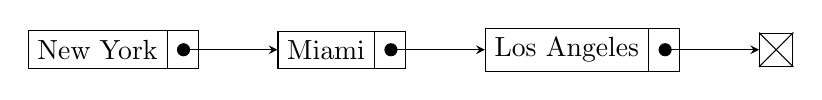
\begin{tikzpicture}[list/.style={rectangle split, rectangle split parts=2,
    draw, rectangle split horizontal}, >=stealth, start chain]

  \node[list,on chain] (A) {New York};
  \node[list,on chain] (B) {Miami};
  \node[list,on chain] (C) {Los Angeles};
  \node[on chain,draw,inner sep=6pt] (D) {};
  \draw (D.north east) -- (D.south west);
  \draw (D.north west) -- (D.south east);
  \draw[*->] let \p1 = (A.two), \p2 = (A.center) in (\x1,\y2) -- (B);
  \draw[*->] let \p1 = (B.two), \p2 = (B.center) in (\x1,\y2) -- (C);
  \draw[*->] let \p1 = (C.two), \p2 = (C.center) in (\x1,\y2) -- (D);
\end{tikzpicture} \\


In the diagram above you can see that each node
contains a data field with the location name presumably as a string. 
Additionally, each node also contains a reference or pointer to 
a the next vertex in the list. The last item of the diagram represents a pointer to 
a null, representing the end of the list. \\


By utilizing the linked list we can begin to construct the graph data structure.
By declaring class Vertex which, contains a data field, as well as a linked list Edges, 
we can add references to every other vertex which said vertex leads to.
By also providing each edge instance with an integer field, weight,
we can therby construct a weighted graph.

If we were to create a bi-directional graph, we could simply add logic which is triggered upon
edge addition to a given vertex, which also creates a pointers in the opposite direction, 
preventing user error and avoiding the accidental creation of a partially non directed graph. \\

\newpage
This can be represented as following, where each node is a vertex, and each arrow leading 
from that vertex is a linked list of edges, each bearing a weight. \\



\begin{figure}[!ht]
\centering

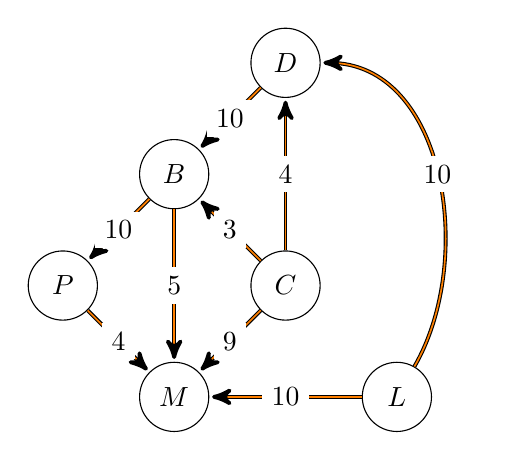
\begin{tikzpicture}[>=stealth',shorten >=1pt,node distance=2cm,on grid,initial/.style    ={}]
  \node[state]          (P)                        {$P$};
  \node[state]          (B) [above right =of P]    {$B$};
  \node[state]          (M) [below right =of P]    {$M$};
  \node[state]          (D) [above right =of B]    {$D$};
  \node[state]          (C) [below right =of B]    {$C$};
  \node[state]          (L) [below right =of C]    {$L$};
\tikzset{mystyle/.style={->,double=orange}} 
\tikzset{every node/.style={fill=white}} 
\path (C)     edge [mystyle]    node   {$3$} (B)
      (D)     edge [mystyle]    node   {$10$} (B) 
      (L)     edge [mystyle]    node   {$10$} (M)
      (B)     edge [mystyle]    node   {$10$} (P);
\tikzset{mystyle/.style={->,double=orange}}   
\path (P)     edge [mystyle]   node   {$4$} (M)
      (C)     edge [mystyle]   node   {$9$} (M) 
      (C)     edge [mystyle]   node   {$4$} (D)
      (B)     edge [mystyle]   node   {$5$} (M);
\tikzset{mystyle/.style={->,relative=false,in=0,out=60,double=orange}}
\path (L)     edge [mystyle]   node   {$10$} (D); 
\end{tikzpicture}

\caption{Graph} \label{fig:M1}
\end{figure}

\subsection{Software and its Presentation, including testing (and video link)}


\subsection{Descriptive Report, including artefacts}

To begin with constructing the artefacts necassary we will first start with the linked list.


\makeatletter
\renewcommand{\ALG@name}{Nested Class}
\makeatother
\setcounter{algorithm}{0}

% =============================================================
\begin{algorithm}
\caption{Node}\label{euclid}
\begin{verbatim}
public class Node {
       Node(T d){
          data = d;
          next = null;
      }
  T data;
  Node next;

  public void setNextNode(Node node) {
      this.next = node;
  }
  public Node getNextNode() {
      return this.next;
  }
 }
\end{verbatim}
\end{algorithm}

We start by first encapsulating a node 
class via class composition inside of our LinkedList. We pass data as
a generic for function composabilitys sake. Each node has a reference field 
to the next node, enabling the linking we seek, as well as a data field.

\newpage

We can now begin our linked list functions. We will continue to pass
generics as arguments to our functions as opposed to specializing to a Vertex data type
for reasons aforementioned. \\

\makeatletter
\renewcommand{\ALG@name}{Function}
\makeatother
\setcounter{algorithm}{0}

% =============================================================
\begin{algorithm}
\caption{Remove If}\label{euclid}

\begin{verbatim}
public void removeIf(Predicate<T> predicate) {
    Node current = head;
    while (current != null) {
        if (predicate.test(current.data)) {
            deleteValue(current.data);
        }
        current = current.next;
    }
}
\end{verbatim}
\end{algorithm}

This function allows us to remove a node from the linked list 
if its data field returns true for a given predicate
which is passed in as an argument to the function. \\

By iterating through each node until we reach null, siginifying
the end of the list, we can then call an additional 
function, deleteValue, if our predicate is met, for each node.

This allows for finer control should we be tasked with deleting 
for example, all nodes which have a string data field value 
beginning with n, or a integer data value less than 10, for e.g.




%=============================================================
\begin{algorithm}
\caption{get}\label{euclid}

\begin{verbatim}
public T get(int index) {
    if (index < 0 || index >= size) {
        throw new IndexOutOfBoundsException(index+" OOB");
    }
    Node current = head;
    for (int i = 0; i < index; i++) {
        current = current.next;
    }
    return current.data;
}
\end{verbatim}

\end{algorithm}

The get function is fairly straight forward and simply allows 
us to retrieve the data of a node at a specified index.
An exception is thrown for the out of bounds case rather than 
printing an error to the user and/or returning null, 
as this allows us to separate the error handling code 
from the normal control flow aiding maintainability.

\newpage
% =============================================================
\begin{algorithm}
\caption{contains}\label{euclid}

\begin{verbatim}
public boolean contains(T element) {
    Node current = head;
    while (current != null) {
        if (current.data.equals(element)) {
            return true;
        }
        current = current.next;
    }
    return false;
}
\end{verbatim}

\end{algorithm}

The contains function is again self explanatory, and simply
iterates though each node until finding the null reference, 
returning true and terminating the function if the list contains
the element passed into the function. \\



% =============================================================
\begin{algorithm}
\caption{peek}\label{euclid}

\begin{verbatim}
public T peek(){
    if (head == null){
    System.out.println("List is empty");
    return null;
  } else {
    return head.data;
  }
}
\end{verbatim}

\end{algorithm}

The peek function takes no arguments and simply returns us the head, 
otherwise informing us that the list is empty should this be true.

\pagebreak


% =============================================================
\begin{algorithm}
\caption{peekEnd}\label{euclid}

\begin{verbatim}
public T peekEnd(){
    if (head == null){
      System.out.println("list is empty");
      return null;
  } else {
    Node current = head;
    while (current.next != null) {
      current = current.next;
    }
    return current.data;
  }
}
\end{verbatim}

\end{algorithm}


Similarly to the last function, this function instead traverses the 
list and returns us the tail of the list, again returning null if 
the list is empty.



% =============================================================
\begin{algorithm}
\caption{pop}\label{euclid}

\begin{verbatim}
public T pop(){
  if (head == null) {
    System.out.println("List is empty");
    return null;
  }
    T value = head.data;
    head = head.next;
    size--;
    return value;
}
\end{verbatim}

\end{algorithm}


The pop function allows us to delete the head of our list, 
decrementing the list size field in the process. 
It maintains the additional linkages by setting the class
head value to be that of head.next. The function also returns 
deleted node to allow for further manipulation.

\pagebreak

% =============================================================
\begin{algorithm}
\caption{popEnd}\label{euclid}

\begin{verbatim}
public MyLinkedList<T> popEnd(){
     if (head == null) {
     System.out.println("List is empty");  
   }
    else{
      if (head.next == null){
        head = null;
        size--;
        
    } else {
      Node current = head;
      while (current.next.next != null){
        current = current.next;
      }
      current.next = null;
      size--;
    }
  }
    return this;
 }
\end{verbatim}

\end{algorithm}


Similarly to the last function, the popEnd function instead allowing
us to delete the tail of the list by first traversing the list,
instead returning the list instance itself.



% =============================================================
\begin{algorithm}
\caption{push}\label{euclid}

\begin{verbatim}
public MyLinkedList<T> push(T data){
    Node newNode = new Node(data);
    if (this.head == null) {
              this.head = newNode;
    } else {
      newNode.next = head;
      head = newNode;
  }
  size++;
  return this;
}
\end{verbatim}

\end{algorithm}

Push allows us to add a new head to the existing list 
with the passed in data argument, setting the previous head 
to head.next to maining our linkage.

\newpage



% =============================================================
\begin{algorithm}
\caption{pushEnd}\label{euclid}

\begin{verbatim}
 public MyLinkedList<T> pushEnd(T data)
  {
      // Instantiate node with argument
      Node newNode = new Node(data);
       
      // check for emptyness, set head if true
      if (this.head == null) {
          this.head = newNode;
      }
      else {
          // traverse the list & insert at the null position
          Node last = this.head;
          while (last.next != null) {
              last = last.next;
          }
          last.next = newNode;
      }
      size++;
      return this;
  }
\end{verbatim}

\end{algorithm}


Similarly, pushEnd allows us to a new node at the end of the list by first starting 
at the head and iterating through each node subsequently until null is found. 
The tail is then pointed to our new node, which then becomes our new tail.
\newpage

%%% =============================================================

\vspace*{0pt}
\begin{algorithm}
\caption{deleteAt}\label{euclid}

\begin{verbatim}
public  MyLinkedList<T> deleteAt(int index)
{
    // Store head node
    Node current = this.head, previous = null;
    // If index == 0, delete head & confirm deletion.
    if (index == 0 && current != null) {
        this.head = current.next; // Changed head
        size--;
        return this;
    }
    // if the index argument < than size of list
    // if counter = argument, connect previous & next
    // then confirm deletion
    // else traverse & increment tracker
    int tracker = 0;
    while (current != null) {
        if (tracker== index) {
            previous.next = current.next;
            size--;
            break;
        }
        else {
            previous = current;
            current = current.next;
            tracker++;
        }
    }
    if (current == null) {
        System.out.println(index + " position element not found");
    }
    return this;
}
\end{verbatim}
\end{algorithm}
The purpose of this function is to delete a node at a given position.
First an emptyness check is performed. If the list is not empty
we iterate through each node until we find our target node. 
We then reassign the previous nodes next field to the targets next.
If a deletion takes place, the size is decremented. \\

It would be wise to update this function to utilize the size field
of the structure to prevent us from iterating through the list 
should we already know that the argument index is our of bounds,
leading to faster run time, though this is not strictly
necassary at this early stage.

\newpage

% =============================================================
\begin{algorithm}
\caption{deleteValue}\label{euclid}

\begin{verbatim}
public MyLinkedList<T> deleteValue(T value)
{
    Node current = this.head, previous = null;
    // check for emptyness. If the head contains the value, delete
    if (current != null && current.data == value) {
        this.head = current.next; 
        System.out.println(value + "has been deleted");
        size--;
        return this;
    }

    // else iterate until val is found or end(null) is reached
    while (current != null && current.data != value) {
        previous = current;
        current = current.next;
    }
    // if iteration stopped before the end, connect previous & next
    if (current != null) {
        previous.next = current.next;
        System.out.println(value + " has been deleted");
        size--;
    }
    
    // if end is reached, value does not exist. 
    if (current == null) {
        System.out.println("this list does not contain" + value);
    }
    return this;
}
\end{verbatim}
\end{algorithm}

This function allows us to delete a value with a specific value 
should it be present in the list. If a node is found with a 
data field corresponding to that of the arguments, we update 
the current.previous next field to point current.next. \\

This function is also utilized as a helper function by the removeIf
function as aforementioned.

\newpage


%% =============================================================
\begin{algorithm}
\caption{getSize}\label{euclid}

\begin{verbatim}
public T removeHead() {
    Node removedHead = this.head;
    if (removedHead == null) {
      return null;
    }
    this.head = removedHead.getNextNode();
    return removedHead.data;
}



\end{verbatim}
\end{algorithm}

This function simply removes the head of the list, 
updates the new head to be the next in the list, 
and returns the data field of the deleted node. \\



%% =============================================================
\begin{algorithm}
\caption{removeHead}\label{euclid}
\begin{verbatim}
public int getSize(){return size;}
\end{verbatim}
\end{algorithm}

This functions requires no explanation.






%=============================================================
\begin{algorithm}
\caption{displays}\label{euclid}
\begin{verbatim}
public void display()
{
    Node current = this.head;
    while (current != null) {
        System.out.print(current.data + " ");
        current = current.next;
    }
    System.out.println("\n");
}
\end{verbatim}
\end{algorithm}

This function iterates through each node of the list 
and displays its data field. As we are a generic for our
data field type, we ought to place guards here to prevent 
us from attempting something which has no means of doing so.
Though, for our use case, this shall suffice for the time being.

\newpage



Finally, as our class implements an Iterator, we must specify 
how we should implement these methods via overloading.


\vspace{6mm}
\makeatletter
\renewcommand{\ALG@name}{Nested Class}
\makeatother
\setcounter{algorithm}{1}


\begin{algorithm}
\caption{Iterator}\label{euclid}
\begin{verbatim}
  private class MyLinkedListIterator implements Iterator<T> {
    private Node current = head;

    @Override
    public boolean hasNext() {
      return current != null;
    }

    @Override
    public T next() {
      T data = current.data;
      current = current.next;
      return data;
      }
    }
  }
  @Override
    public Iterator<T> iterator() {
      return new MyLinkedListIterator();
    }
\end{verbatim}
\end{algorithm}
\vspace{8mm}


The purpose of this class is to provide an iterator object that can be used to iterate over the of a list.
The use case of these functions will soon be discussed.\\

The hasNext function returns a boolean indicating whether there are elements remaining in the collection to be iterated over,
by checking if null has been reached at which point false is returned. \\

The next function returns the next node in the list by
returning the data stored in the current node and setting current to the next node in the list.
An exception is then thrown should next be null. \\

Finally a constuctor is defined to allow us to instiate an instance of the nested class for usage. \\

\newpage




\vspace{6mm}
\makeatletter
\renewcommand{\ALG@name}{Class}
\makeatother
\setcounter{algorithm}{1}

This class allows us to extend the functionality of our 
node type. As we incorperated generic types into our linked list arguments,
we can now create a LinkedList field of type Edge, (soon to discuss) for our Vertex.


\vspace{12mm}

\begin{algorithm}
\caption{Vertex}\label{euclid}
\begin{verbatim}
public class Vertex {
  private String data;
  private MyLinkedList<Edge> edges;
  }
\end{verbatim}
\end{algorithm}

\makeatletter
\renewcommand{\ALG@name}{Vertex Function}
\makeatother
\setcounter{algorithm}{0}


\vspace{6mm}


\begin{algorithm}
\caption{Constructor}\label{euclid}
\begin{verbatim}
  public Vertex(String data){
    this.data = data;
    this.edges = new MyLinkedList<Edge>();
  }
\end{verbatim}
\end{algorithm}


\vspace{6mm}

\begin{algorithm}
\caption{getData}\label{euclid}
\begin{verbatim}
  public String getData(){
  return this.data;
  }
\end{verbatim}
\end{algorithm}
\newpage


\begin{algorithm}
\caption{getedges}\label{euclid}
\begin{verbatim}
  public mylinkedlist<edge> getedges(){return this.edges;}
\end{verbatim}
\end{algorithm}




\begin{algorithm}
\caption{addEdge}\label{euclid}
\begin{verbatim}
  public void addEdge(Vertex to, int weight){
    this.edges.push(new Edge(this, to, weight));
  }
\end{verbatim}
\end{algorithm}

\vspace{4mm}

The addEdge function allows us to create a new edge for a Vertex,
by passing in a reference to the calling Vertex, aswell as a to Vertex,
which is used to denote the destination. Additionally we pass in the weight of the edge.


\vspace{4mm}
\begin{algorithm}
\caption{deleteEdge}\label{euclid}
\begin{verbatim}
  public void deleteEdge(Vertex rhsTo){
    this.edges.removeIf(edge -> edge.getTo().equals(rhsTo));
  }
\end{verbatim}
\end{algorithm}


This calls the aforementioned removeIf function using a reference to 
the calling Vertex as well as an argument destination Vertex as a predicate, 
deleting the edge if the edge exists.

\newpage


\vspace*{0pt}

\begin{algorithm}
\caption{print}\label{euclid}
\begin{verbatim}
  public void print(boolean showWeight){
    String toPrint = "";
    if(this.edges.getSize() == 0){
      System.out.println(this.data + "-->");
      return;
    }

    for(int i =0; i<this.edges.getSize(); i++){

      if (i == 0){
        toPrint += this.edges.get(i).getFrom().data + "-->";
      }
      toPrint += this.edges.get(i).getTo().data;

      if(showWeight){
        toPrint += " (" + this.edges.get(i).getWeight() + ")";
      }
      if (i != this.edges.getSize() -1){
        toPrint += ", ";
      }
    }
    System.out.println(toPrint);
  }
}
\end{verbatim}
\end{algorithm}

\vspace{4mm}

This function allows us to display all the edges of a given vertex,
additionally including a boolean parameter which can be used to specify 
whether weighing for each should be shown. This allows for flexibility in the 
ways in which we display our data and prevents us from unnecessarily
overloading the function.
\newpage




% ==========================  Edge ========================= 

\vspace{6mm}
\makeatletter
\renewcommand{\ALG@name}{Class}
\makeatother
\setcounter{algorithm}{2}



\begin{algorithm}
\caption{Edge}\label{euclid}

\begin{verbatim}
public class Edge {

  private Vertex from;
  public Vertex getFrom() {
    return from;
  }

  private Vertex to;
  public Vertex getTo() {
    return to;
  }

  private Integer weight;
  public Integer getWeight() {
    return weight;
  }

  public Edge(Vertex fromVertex, Vertex toVertex, Integer weight){
    this.from = fromVertex;
    this.to = toVertex;
    this.weight = weight;
  }
}
\end{verbatim}
\end{algorithm}

This class is fairly self explanatory and simply contains three fields.
From contains a starting Vertex, to contains a destination Vertex,
and finally weight. 
\newpage

\begin{algorithm}
\caption{Graph}\label{euclid}

\begin{verbatim}
public class Graph {
  
  private MyLinkedList<Vertex> vertices;
  public MyLinkedList<Vertex> getVertices() {return vertices;}

  private boolean isGraphWeighted;
  public boolean isGraphWeighted() {return isGraphWeighted;}

  private boolean isGraphDirectional;
  public boolean isGraphDirectional() {return isGraphDirectional;}

  public Graph(boolean setIsGraphWeighted, boolean setIsGraphDirectional){
    this.vertices = new MyLinkedList<Vertex>();
    this.isGraphWeighted = setIsGraphWeighted;
    this.isGraphDirectional = setIsGraphDirectional;
  }
\end{verbatim}
\end{algorithm}

\vspace{8mm}

Finally we have the graph class itself. Storing a linked list of vertices aside,
the class is fairly unremarkable besides
the inclusion of two boolean fields, isGraphWeighted, and isGraphDirectional. \\

These fields allow us to specify the type of our graph once upon initialization,
and the proceding functions use those values accordingly to spare us either passing around null values,
or writing seperate implementations of the Graph class for our use case. This extensibility may well
prove useful down the line.



\newpage
\begin{verbatim}
public Vertex addVertex(String data){
    Vertex newOne = new Vertex(data);
    this.vertices.pushEnd(newOne); // push start or end?
    return newOne;
  }
  public void addEdge(Vertex from, Vertex to, Integer weight){
    if (!this.isGraphWeighted){
      weight = null;
    }
    from.addEdge(to, weight);
    if (!this.isGraphDirectional){
      to.addEdge(from, weight);
    }
  }
  public void deleteEdge(Vertex from, Vertex to){
    from.deleteEdge(to);
    if (!this.isGraphDirectional){
      to.deleteEdge(from);
    }
  }
  public void deleteVertex(Vertex vertex){
    this.vertices.deleteValue(vertex);
  }
  public Vertex getVertexWithVal(String val){
    for(Vertex v : this.vertices){
      if (v.getData() == val) {
        return v;
      }
    }
    return null;
  }
  public void print() {
    for(Vertex each : this.vertices){
      each.print(isGraphWeighted());
    }
  }

\end{verbatim}

The usage of these boolean attributes can be seen here, the most noteworthy being addEdge.
This function handles setting weight to null for each vertex to ensure consistency.
Additionally, if we set isGraphDirectional to false, an edge pointer will be added to the
start Vertex to the end Vertex, as well as from the end Vertex, to the start Vertex, denoted by from and to respectivly.
further preventing inconsistncy. Furthermore, should we need to create a graph in which only some edges are directed, 
we could overload the addEdge function to also take a boolean argument to determine whether that edge is directional.

\newpage



  

% ========================================================== 
\subsubsection{Transitioning algorithms to implementation}

We can now begin implementing our algorithms by first populating our graph. \\


\begin{verbatim}
    Graph usa = new Graph(true, true);
    Vertex newYork = usa.addVertex("New York");
    Vertex chicago = usa.addVertex("Chicago");
    Vertex denver = usa.addVertex("Denver");
    Vertex dallas = usa.addVertex("Dallas");
    Vertex miami = usa.addVertex("Miami");
    Vertex sanFran = usa.addVertex("San Fran");
    Vertex sanDiego = usa.addVertex("San Diego");
    Vertex losA = usa.addVertex("LA");

    usa.addEdge(newYork, chicago, 75);
    usa.addEdge(newYork, denver, 100);
    usa.addEdge(newYork, dallas, 125);
    usa.addEdge(newYork, miami, 90);
    usa.addEdge(chicago, sanFran, 25);
    usa.addEdge(chicago, denver, 20);
    usa.addEdge(miami, dallas, 50);
    usa.addEdge(dallas, losA, 80);
    usa.addEdge(dallas, sanDiego, 90);
    usa.addEdge(denver, sanFran, 75);
    usa.addEdge(denver, losA, 100);
    usa.addEdge(sanDiego, losA, 45);
    usa.addEdge(sanFran, losA, 45);
\end{verbatim}




\vspace{12mm}

We will first start with depth first search, which is simple to implement but gives
us no guarantees that any path we find will result in the lowest possible edge weight sum 
for the completed path, as there is no heuristics involved. For simplicitys sake we will follow our ADl logic and focus on the traversal 
steps, before adapting the algorithm to return the results that we desire.

\newpage

 


\begin{algorithm}
\caption{Depth First Traversal}\label{euclid}

\begin{verbatim}
public static void depthFirstTraversal(
Vertex startV, MyLinkedList<Vertex> visitedList){

    for(Edge e : startV.getEdges()){
      Vertex thisNeighbour = e.getTo();

      if (!visitedList.contains(thisNeighbour)){
        visitedList.push(thisNeighbour);
        Traverser.depthFirstTraversal(thisNeighbour, visitedList);
      }
    }
  }
\end{verbatim}
\end{algorithm}


\vspace{12mm}







To begin, a linked list to store visited vertices, visitedList 
is passed in rather than declared within the function,
to allow us to make use of the call stack recursivly. \\

We start by iterating through each edge of the starting Vertex,
storing the vertex as thisNeighbour. 
If visitedList does not contain thisNeighbour,
we add thisNeighbour to the visitedList. \\

We then recursively call the depthFirstTraversal function with thisNeighbour as 
the starting vertex and the updated visitedList. \\

We continue exploring the graph in this manner, 
pushing our function calls onto the cll stack passing the next neighbouring vertex.
When the function has finished processing the current vertex and all its neighbors, 
the function call is popped off the call stack and the program continues with the next function call on the stack
until there are no more unvisited vertices.
This will lead us to have visited all vertices in the graph which the starting vertex is connected to directly and/or indirectly.\\
Once the call stack is empty, the function terminates. \\
\newpage




\begin{algorithm}
\caption{Depth First Search}\label{euclid}

\begin{verbatim}
  public static void depthFirstSearch
  (Vertex startV, Vertex endV, MyLinkedList<Vertex> visitedList, 
  MyLinkedList<Vertex> path, int totalWeight){
    path.push(startV);

    if (startV.equals(endV)){

      for(Vertex v : path) {
        if(v != endV){
        System.out.print(v.getData() + " -> ");
        } else {System.out.println(v.getData());}
      }

      System.out.println(
        "This journey has a total weight of: "+totalWeight);

    } else {
        for(Edge e : startV.getEdges()){
            Vertex thisNeighbour = e.getTo();

            if (!visitedList.contains(thisNeighbour)){
              visitedList.push(thisNeighbour);
              Traverser.depthFirstSearch(
                thisNeighbour, endV, visitedList, path, 
                totalWeight + e.getWeight());
            }
          }
        }
      //remove current vertex from path before returning
      path.deleteAt(path.getSize() -1);
    }


\end{verbatim}
\end{algorithm}

By also passing a desired end Vertex, a weight integer, as well as an addtional linked list
We can construct a path while accumulating our edge weight sums for said path.

We start by pushing the starting Vertex onto our path,
before checking that we have not yet reached the target Vertex.
If so we iterate through each Vertex within the path printing its data field using its getData method.
Otherwise the function operated much like the traversal, besides the fact we are now passing more parameters 
to our call stack. 
\newpage



\vspace{10mm}
One advantage of using the call stack to implement this  algorithm is that it allows the function to be implemented in a 
fairly simple manner, as the problem lends itself well to a recursive structure,
however, if the graph is very large, or the recursion is very deep, the call stack could potentially consume an extreme amount of memory,
when the problem does not strictly require memoization.
This could lead to less performant code, and eventually a stack overflow. \\
\vspace{4mm}

Recursive algorithms can also be comparativly difficult to debug compared to iterative algorithms as
it can be harder to fully understand the state of the program at each point of execution. \\
\vspace{4mm}

Recursive algorithms can also be slower than iterative algorithms because they involve the overhead of function calls and the maintenance of the call stack.
Furthermore, while on some occastions a compiler can optimize a recursive algorithm, this is not always the case. 
Imperative algorithms are typically 
easier for the compilier to optimize due the imperative nature of assembly.
Additionlly tail call optimization is difficult for the JVM due to the necessity to always have a stack trace available. \\
\vspace{4mm}

Overall, whether recursion is an appropriate choice for implementing this algorithm will depend on 
the specific requirements and constraints of the problem at hand. \\
\newpage
\begin{algorithm}
\caption{Dijkstra Traversal}\label{euclid}

\begin{verbatim}
  public static HashMap[] dijkstra(Graph graph, Vertex startV) {

        HashMap<String, Integer> distTable = new HashMap<>();
        HashMap<String, Vertex> prevTable = new HashMap<>();
        PriorityQueue<PQObj> queue = new PriorityQueue<PQObj>();
        queue.add(new PQObj(startV, 0));

        for (Vertex v: graph.getVertices()) {
            if (v != startV) {
                distTable.put(v.getData(), Integer.MAX_VALUE);
            }
            prevTable.put(v.getData(), new Vertex("Null"));
        }

        distTable.put(startV.getData(), 0);

        while (queue.size() != 0) {
            Vertex current = queue.poll().vertex;
            for (Edge e: current.getEdges()) {
                Integer alt = distTable.get(
                  current.getData()) + e.getWeight();
                String neighbour = e.getTo().getData();
                if (alt < distTable.get(neighbour)) {
                    distTable.put(neighbour, alt);
                    prevTable.put(neighbour, current);
                    queue.add(new PQObj(
                      e.getTo(), distTable.get(neighbour)));
                }
            }
        }
        return new HashMap[]{distTable, prevTable};
    }
\end{verbatim}
\end{algorithm}
\vspace{7mm}

By utilizing Dijkstas's algorithm, we can ensure that the path we have found is indeed the shortest, 
by accumulating the weights for each possible route, and returning the one which has the smallest value. \\

We make use of a priority queue for this algorithm for which we have a custom priority queue object 
which we can pass to our queue strucure, extending it's functionallity. Futher aiding function composability. \\
\newpage

It also utizile two HashMaps to represent tables used to store the distance from the start vertex 
to each vertex and the previous vertex in the shortest path from the start vertex to the current vertex. \\

\vspace{8mm}
\begin{itemize}
\item 
We begin by adding the start vertex and a distance of 0 to the priority queue.
We then initialize the distances table as well asthe previous vertex table for all vertices in the graph,
setting the distance for all vertices except the start vertex to the maximum value to represent infinity,
and the previous vertex for all vertices with null. 

\item
We then enter a loop that continues.
until the priority queue is empty.
With each iteration,
we remove the vertex with the smallest distance from the start vertex from the queue
and examine its neighbours. 

\item
For each neighbouring vertex, we calculate the total weight from the start vertex to the neighbor
by adding the weight of the edge connecting the current vertex to the neighbor,
to the distance of the current vertex from the start vertex. \\

\item
If this distance is less than the current distance recorded in the distance table for the neighbor,
the distance and previous vertex for the neighbor are updated in the distance
and previous vertex tables, and the neighbor is added to the priority queue. \\

\item
Once the loop is finished, the distance table and previous vertex table
will contain the shortest distances from the start vertex to all other vertices in the graph
and the previous vertices on the shortest paths, respectively.
The algorithm returns these tables as an array of HashMap objects. \\
\end{itemize}
\vspace{20mm}

On the following page we will discuss the usage of a function which we will use 
to return the shortest path between any given pair of vertices. 

\newpage


\begin{algorithm}
\caption{Dijkstra Traversal}\label{euclid}

\begin{verbatim}
   public static void shortestPath(
   Graph g, Vertex startV, Vertex endV) {
        HashMap[] tables = dijkstra(g, startV);
        HashMap distances = tables[0];
        HashMap previous = tables[1];

        Integer distance =
          (Integer)distances.get(endV.getData());
        System.out.println(
          "Shortest Distance between "
          + startV.getData()
          + " and " + endV.getData());
          System.out.println(distance);

        MyLinkedList<Vertex> path = new MyLinkedList<>();
        Vertex v = endV;

        while (v.getData() != "Null") {
            path.addAtIndex(0, v);
            v = (Vertex) previous.get(v.getData());
        }
        System.out.println("Shortest Path");
        for (Vertex pathVertex: path){
            System.out.println(pathVertex.getData());
        }
    }
\end{verbatim}
\end{algorithm}


\vspace{6mm}
We pass three arguments to this function,
the starting vertex, the end vertex, as well as our graph.
We then initialize an array of Hashmaps and call our traversal function to populate said array.
We then name each of our array instances with respectively for the sake of code clarity,
before printing the distance from the starting vertex to the target vertex. \\

We then initialize a path to store the vertices in the shortest path.
We then set a Vertex, v, to be equal to the target vertex.

before entering a while loop that continues until our end Vertex is equal to null.
For each iteration of the loop we add the current value of v to the front of the path, 
and set v to be equal to the previous vertex in the shortest path from the starting vertex to v, as stored in the previous table. \\

Finally, we iterate through the path list, printing out the data field of each vertex in the path.




\newpage
\subsubsection{Problem-solving strategy}


\subsection{Incorporation of formative feedback}


\newpage
%========================================================================================%



%========================================================================================%
\section{Project 4}
\subsection{Introduction}
To begin solving our problem we must first contextualize the true meaning of our problem.
The question at hand is truly how can we split a random set of numbers,
so that the difference between the sum of the sets is as minimal as feasible, 
without exhaustively checking every possible configuration. \\

As we are working with a given unit, bricks, we can disregard the complexity of decimals and negative values,
and simply focus on the natural numbers.

\subsubsection{Weights and Load Problem}
The most optimal solution will differ depending upon the characteristics of the numbers in the set,
i.e. 

\begin{itemize}
  \item Are there any patterns within the set? (e.g. all primes)
  \item How large is there range of the set?.

\end{itemize}
\vspace{4mm}

We can not optimize for every circumstance, 
but we can generalize. \\
\vspace{4mm}

The problem is expected to become
incredibly difficult with large sample sized sets, and we are therefore more likely to become more accepting of
a less than optimal solution, that is, a solution which is not the global maximum. 
Furthermore, without using a brute force approach, 
(calculate the sum of every combination of numbers), which would prove prohibitively costly,
if we do not cease iteration using via evaluation of a fitness value  derived from a fitness function,
there is a probability that
we would continue indefinitely, 
never reaching a global maximum, expressed as a worst case time complexity of $(O(\infty)).$ \\

Additionally, preprocessing could be prohibitive in larger sets, and if we intend to use a tree
like structure, we have to consider the effect of pre-processing the input set on the balance of our structure. \\

One approach may be to first pre-process our set by adapting divide and conquer strategy, we can then
begin implementing our 
strategy with an already reasonably distributed set. This strategy would involve sorting the numbers in ascending order before
continually selecting the central element and placing it in the sub-set with the smallest current sum.
This will ensure that the difference between the sums of the two sets is minimized and increases the chance of 
a fitness which is within an acceptable threshold without the need for additional processing. \\

It is important to note that this method does not always guarantee that the difference between the sums of the two sets will be minimized, 
but it is a good starting point and will often produce good results, while also being efficient with regards to time complexity, ($O(n)).$ \\

We may begin by deriving a heuristic front the set. For this, we can first 
halving the sum of all numbers in the original set.
Should this be a whole number, we know that if there exists any configuration of numbers which 
sums to this target then that would be an optimal splitting of the sets.
Should the original set sum be an odd number, we can simply use integer division, 
wherein the 0.5 decimal value will be discarded, and also consider the target plus one to be valid.\\

We must decide whether to terminate our computation after a given length of time, 
after a certain threshold has been met, i.e within 10\% of the target,
or once we have established we have hit a local maximum.
We shall initially aim try to achieve a combination of these three approaches, by running for a set time, 
and ceasing execution if at any point we believe we have reached a local maximum, at which point
we will decide whether to attempt to further process depending on whether we are within a certain threshold of the target.\\

\vspace{8mm}
\subsubsection{The Problem Proposed Solution and Data Structure}

\vspace{4mm}
The initial proposal is as follows;

\vspace{2mm}
\begin{itemize}
  \item Sort starting set by value. Data type must allow for multiples and be ordered.
  \item Create two subsets of an ordered data structure, again multiples must be allowed.
        Track their sums with a int field.
  \item Populate the structures by distributing the original set using a divide and conquer approach.

  \item Enter a loop which continues until either a global maximum has been found, 
    or our fitness is below a set threshold.
  \item Begin small change strategy, placing the target floor value of the larger subset.

  \item If there is no value lower than the target present in the smaller set,
    randomly mutate by arbitrarily moving a number of values.

  \item Repeat until; A global maximum is found, a number of iterations has been surpassed,
    or a fitness value within a given threshold is found.
\end{itemize}
\newpage

As our subsets require to both maintain order, as well as be reasonably efficient to search for the target floor upon each iteration of the random mutation,
we shall use a Tree Map. This will generally provide us with $O(logn)$ time complexity, due to the nature of binary search. 
There is a possibility that our time complexity may decay to $O(n)$ if all of the nodes enter one branch of the tree,
efficiently forming a linked list. This is known as the chain problem. 
By distributing our original set from the centre out we can prevent the likelihood of this occurring.
While we do run the risk of our tree becoming unbalanced, we are unable to utilize hashing.
By storing each node as a key value pair, we can increment the value of our key to allow for repeated integers. 
\vspace{4mm}


\begin{figure}[!ht]
\centering
\vspace{8mm}
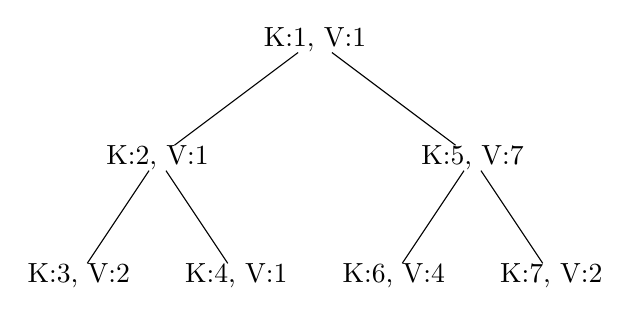
\begin{tikzpicture}[
  level distance=15mm,
  every node/.style={align=center, inner sep=0},
  level 1/.style={sibling distance=40mm},
  level 2/.style={sibling distance=20mm},
  level 3/.style={sibling distance=10mm}
]
\node {K:1, V:1}
  child { node {K:2, V:1}
    child { node {K:3, V:2} }
    child { node {K:4, V:1} }
  }
  child { node {K:5, V:7}
    child { node {K:6, V:4} }
    child { node {K:7, V:2} }
  };
\end{tikzpicture}
\caption{TreeMap} \label{fig:M1}
\end{figure}



\vspace{12mm}
\subsection{Heuristic Optimisation}

To improve the results of our mutation, We can use the following additional heuristic.
On each iteration, we will check if the larger set contains a value equal to the target,
This shall be the predicate of our second heuristic.
If the predicate is true so, make the swap and exit. This may reduce our effective run time,
especially in cases where there is no global maximum, but it does improve our chances of finding it if possible. \\



\newpage
\subsubsection{Designed Fitness Function}

\makeatletter
\renewcommand{\ALG@name}{Fitness Function}
\makeatother
\setcounter{algorithm}{0}

\begin{algorithm}
\caption{Fitness Function}\label{euclid}

\begin{verbatim}
public static double fitnessFunction
(int aSum, int bSum, int target, int brickSum) {
  try {
      if (!isEven(brickSum)) {
          if (aSum == target || aSum == target + 1 
          || bSum == target || bSum == target + 1) return 0;
      } else {
          if (aSum == target || bSum == target) return 0;
      }
      return diffAsPosiPerc(smallestDiff(aSum, bSum, target), target);
  } catch (Exception e) {
      System.out.println(
      "An error occurred while calculating the fitness function: " 
      + e.getMessage());
      return 0;
  }
}
\end{verbatim}
\end{algorithm}
\vspace{4mm}

This fitness function utilizes function composition to return the fitness of the function
defined as the difference between the target/s and the sub set sum with the smallest difference.
The functions it is comprised of are written with referential transparency in mind to aid in 
testing.


\vspace{8mm}
\begin{algorithm}
\caption{Fitness Evaluation}\label{euclid}

\begin{verbatim}

public static boolean fitnessEvaluator(double fitness){
      return fitness < 0.3 ? true : false;  
  }
\end{verbatim}
\end{algorithm}
\newpage






\vspace{8mm}
\subsubsection{Introduction to Hill Climbing}
Hill climbing algorithms are a class of optimization algorithms that are used to find the maximum or minimum value of a function.
These algorithms are called "hill climbing" because they operate by iteratively making small changes to the input of the function in an effort 
to "climb" to the highest (or lowest) point on the function's curve. \\

Hill climbing algorithms are generally simple to implement and can be effective at finding good, 
local solutions to optimization problems. 
However, they can sometimes get stuck in local optima, 
meaning that they may not find the global maximum or minimum of the function. 
There are many variations of hill climbing algorithms,
including simple hill climbing, steepest ascent hill climbing, and simulated annealing.
These algorithms can be applied to a wide range of optimization problems, including finding the shortest path between two points, 
fitting a model to data, and many others. \\

Overall, hill climbing algorithms are a useful tool for finding good solutions to optimization problems,
but they may not always find the absolute best solution. \\


\subsubsection{Small Change Strategy}

\makeatletter
\renewcommand{\ALG@name}{Small Change}
\makeatother
\setcounter{algorithm}{0}


\begin{algorithm}
\caption{Transfer Smallest Value of Largest Subset}\label{euclid}

\begin{verbatim}
procedure smallChange(
    lhs: TreeMap[int, int], rhs: TreeMap[int, int], 
    lhsSum: int, rhsSum: int, target: int) -> bool:

    lhs increment(rhs first value)
    lhsSum += (rhs first value)
    rhsSum -= (rhs first value)
    rhs decrement(rhs first value)
    
    if (targetFound)
      return True
    else
      return False 
    
end procedure
\end{verbatim}
\end{algorithm}

By continually shifting the smallest value of the larger a subset, 
a high level of fidelity can be achived. This is an alternative to 
continually traversing the tree on every iteration to find a value closest to 
the target. Used in conjunction with the random mutation, we can very quickly arrive at a close 
approximation of the global maximum at very little computational cost. 


\subsection{Incorporation of Formative Feedback}

\newpage
%========================================================================================%


%========================================================================================%
\section{Project 5}

\subsection{Experiment Strategy}
\vspace{8mm}
To better understand the real run time implications of our implementation 
we must define metrics in which to test a number of variables against. and determine
our control methods.\\

% he independent variable is the factor that is being manipulated or changed in the experiment.
% It is the cause in the cause-and-effect relationship being studied.

% The dependent variable is the outcome that is being measured in the experiment. 
% It is the effect in the cause-and-effect relationship.

% The control is a standard against which the other variables are compared
% . It helps to isolate the effect of the independent variable on the dependent variable by holding all other variables constant.

We aim to analyse the effectiveness of our algorithm as a whole, as well as the bearing of
changes that we make. For this reason we will contrast and compare the addition of
the random mutation on our algorithm. \\

We will run each variant of the program $100$ times, taking the mean of the 
final fitness of each set of 10 iterations, before recording our tabulating our results, 
and subsequently plotting them on line chart for ease of comparison. \\

It is imperative that we isolate the effect of the independent variable on the dependant variable 
by holding all other variables constant. Therefore we will ensure that both variants of the program
recieve the same inputs as arguments\\



\vspace{12mm}

\begin{itemize}
  \item \textbf{Independant Variable} We will contast the use and non use of random mutation
    to highlight the concept of local optima.
\end{itemize}

\begin{itemize}
  \item \textbf{Dependant Variable:} We will take the mean fitness of each 10 iterations
    measured in \% difference from the target.
\end{itemize}

\begin{itemize}
  \item \textbf{Control:} We will ensure both programs will take the same arguments as input, 
    and both will be ran 100 times and averaged.
\end{itemize}



  
\newpage
\subsection{Experiment Results}

\begin{figure}[h]
  
\centering
  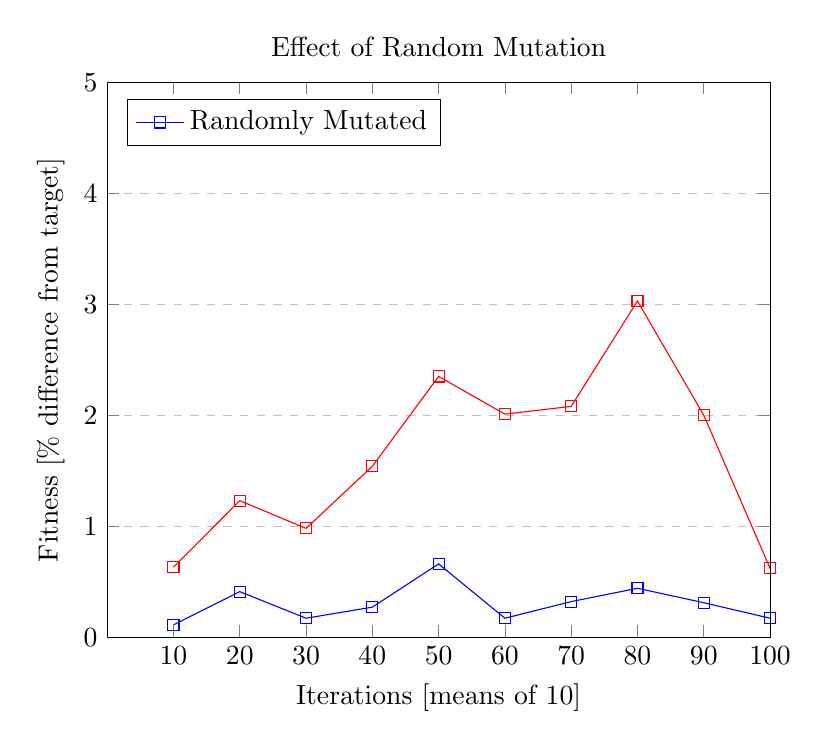
\begin{tikzpicture}
  \begin{axis}[
    title={Effect of Random Mutation},
      xlabel={Iterations [means of 10]},
      ylabel={Fitness [\% difference from target]},
      xmin=0, xmax=100,
      ymin=0, ymax=5,
      xtick={10,20,30,40,50,60,70,80,90,100},
      ytick={0,1,2,3,4,5},
      legend pos=north west,
      ymajorgrids=true,
      grid style=dashed,
  ]

  \addplot[
      color=blue,
      mark=square,
      ]
      coordinates {
      (10,0.11)(20, 0.41)(30, 0.17)(40, 0.27)(50, 0.66)(60, 0.17)(70, 0.32)(80, 0.44)(90,0.31)(100,0.17)
      };
      \legend{Randomly Mutated}

  \addplot[
      color=red,
      mark=square,
      ]
      coordinates {
      (10,0.63)(20,1.23)(30,0.98)(40,1.54)(50,2.35)(60,2.01)(70,2.08)(80,3.03)(90,2.00)(100,0.62)
      };
  \end{axis}
  \end{tikzpicture}
\caption{Sample size of $20$}
\label{fig:x Mutation Plot}

\end{figure}

\subsection{Discussion}

It can be seem from the figure above that the incluson of random mutation within
the algorithm consistently achieved much better results. \\

Both variants of the algorithm perform fairly adequetly considering the
worst of 3\% within the target for the non-mutated variant. \\

Depending on requirments, as well as the size of the dataset,
it could in some cases be preferable to simply aim 
to reach a local maxima and cease execution there. 
As our dataset is relatily small, the somewhat costly tree traversal required
to randomly select values is arguably justafied. \\

Of course the brute force exhaustive search not be ideal, even with a data set of this size. 
There $(2^n)$ different ways to place $n$ numbers into two sets.
for our sample size of 20 it would take significantly 
more than 1048576 operations to calculate every configuration,
since each operation would involve at least one comparison and one assignment,
and these operations would have to be repeated for each number in the set.



\newpage



\subsection{Largest Dataset Experiment}


\subsubsection{Dataset}

For this experiment, random numbers within the range of the previous and maximum size 
of the previous dataset. Rather than the $20$ that were used previously, we will instead 
generate $2000$.

\subsubsection{Results}

\begin{figure}[h]
  
\centering
  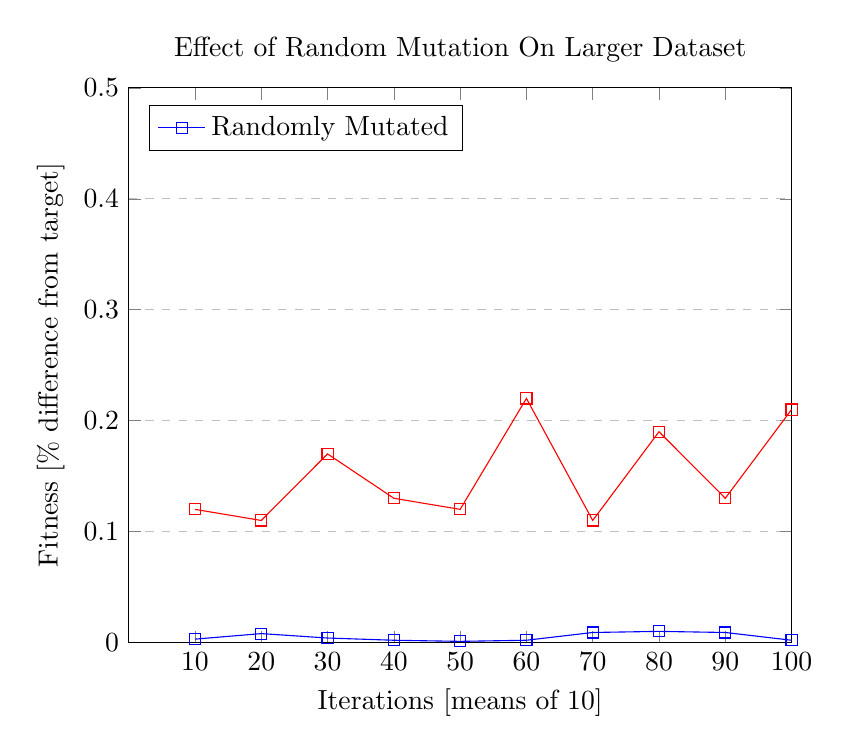
\begin{tikzpicture}
  \begin{axis}[
    title={Effect of Random Mutation On Larger Dataset},
      xlabel={Iterations [means of 10]},
      ylabel={Fitness [\% difference from target]},
      xmin=0, xmax=100,
      ymin=0, ymax=0.5,
      xtick={10,20,30,40,50,60,70,80,90,100},
      ytick={0,0.1,0.2,0.3,0.4,0.5},
      legend pos=north west,
      ymajorgrids=true,
      grid style=dashed,
  ]

  \addplot[
      color=blue,
      mark=square,
      ]
      coordinates {
      (10,0.003)(20, 0.008)(30, 0.004)(40, 0.002)(50, 0.001)(60, 0.002)(70, 0.009)(80, 0.01)(90,0.009)(100,0.002)
      };
      \legend{Randomly Mutated}

  \addplot[
      color=red,
      mark=square,
      ]
      coordinates {
      (10,0.12)(20,0.11)(30,0.17)(40,0.13)(50,0.12)(60,0.22)(70,0.11)(80,0.19)(90,0.13)(100,0.21)
      };
  \end{axis}
  \end{tikzpicture}
\caption{Sample size of 2000}
\label{fig:x Mutation Plot}

\end{figure}

\subsubsection{Discussion}

It is evident from the results that both the mutated and non mutated variants
of the algorithms perform favourably when presented with a larger data set. \\

This is most likely due to the fact that the algorithm performed a check for 
a global maxima.
The larger dataset results in a larger configurations of numbers,
and thus the likelyhood of finding at any stage a value which 
corresponds to the target is signifigantly increased. \\

It can be seen in the non mutated variant, that while the inability to deviate from
a local maxima does negativly impact the resulting fitness, the previous statement is still true, 
in that the increased fidelity allows us to incidentally find a value closer to the target.


% \subsection{Testing}

\newpage
\subsection{Software and its Presentation, including testing (and video link)}
\vspace{4mm}
The program consists of 6 distinct steps, namely;
\vspace{4mm}
\begin{enumerate}
  \item \textbf{Initialization:} This path includes the creation of the bricks list and the assignment of random values to it.
  \item \textbf{Distribution:} This path includes the distribution of the bricks into the a and b TreeMaps.
  \item \textbf{Small Change:} This path includes the transfer of TreeMap key floors.
  \item \textbf{Mutation:} This path includes the random mutation of elements between the a and b TreeMaps.
  \item \textbf{Evaluation:} This path includes the evaluation of the fitness of the current configuration of the a and b TreeMaps.
  \item \textbf{Termination:} This path is taken when the program terminates, either because the target sum has been reached or the maximum number of iterations has been reached.
  \end{enumerate}

\vspace{4mm}

  

The cyclomatic complexity of a function takes into account only the independent paths within the function itself, 
not the paths taken through any functions that it calls. \\

because it only has one independent path (the return statement). 
For example, the cyclomatic complexity of the incrementMapVal function is 2.
and can be expressed formally as
$M = E - N + 2P = 2 - 1 + 2 * 1 = 2$. \\

However, the isEmpty and contains methods, which are called by incrementMapVal function,
have their own cyclomatic complexities based on the independent paths within those functions. \\


\begin{figure}[h!]
\centering
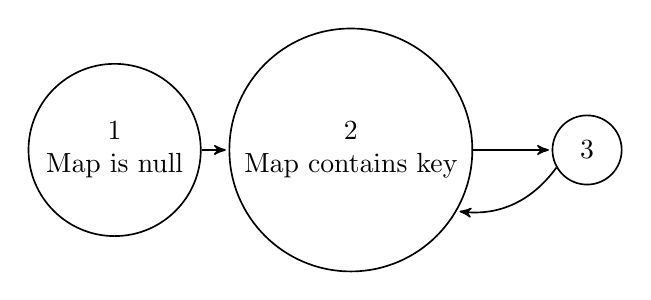
\begin{tikzpicture}[->,>=stealth',shorten >=1pt,auto,node distance=3cm,
                    semithick,
                    every node/.style={align=center}]
  \tikzstyle{every state}=[draw=black,text=black]

  \node[state] (1) {1\\Map is null};
  \node[state] (2) [right of=1] {2\\Map contains key};
  \node[state] (3) [right of=2] {3};

  \path (1) edge (2)
        (2) edge (3)
        (3) edge [bend left] (2);
\end{tikzpicture}
\end{figure}



To calculate the overall cyclomatic complexity of the program,
we would need to sum the cyclomatic complexities of all the functions in the program, 
including any functions that they call. \\








% ======================================================================================
\newpage
\begin{figure}[!h]
\vspace*{-1.5cm} 
\caption{Mcgabes Cyclomatic Complexity Flow Chart for Hill Climb Algorithm}
\label{fig:x mainflow}
\vspace{7mm}

\tikzset{decision/.style={ % requires library shapes.geometric
        draw,
        diamond,
        aspect=3,
        node distance= 2.5cm
    }}
\def\minhg{10cm}
\def\minwd{5cm}

\tikzstyle{block} = [rectangle, draw,text width=5em, text centered, rounded corners, minimum height=4em]
\tikzstyle{dec} = [diamond, draw,text width=5em, text centered, rounded corners, minimum height=4em]
\tikzstyle{line} = [draw, very thick, color=black!50, -latex']
\tikzstyle{cloud} = [draw, ellipse,fill=red!20, node distance=2.5cm,minimum height=2em]

\hspace*{-2cm} 
\begin{tikzpicture}[scale=2, node distance = 2cm, auto]

    \node [block] (init) {Initialize};
    \node [block, below of=init] (start) {Start Iteration};
    \node [decision, below of=start] (global) {Global Maxima Found?};
    \node [block, below of=global] (smallch) {Small Change};
    \node [decision, below of=smallch] (zerochange) {No Change?};
    \node [decision, below of=zerochange] (bestfitness) {Best Fitness?};
    \node [decision, below of=bestfitness] (threshold) {Within Threshhold?};
    \node [decision, below of=threshold] (itercount) {Iteration count Exceeded?};
    \node [block, below of=itercount] (terminate) {Terminate};
    
    \node [block, left of=global, node distance=7cm] (ss) {Save State};
    \node [block, left of=zerochange, node distance=5cm] (mutate) {Mutate};
    \node [block, left of=bestfitness, node distance=5cm] (savestate) {Save State};

    \path [line] (init) -- (start);
    \path [line] (start) -- (global);
    \path [line] (global) -- node [near start] {no}(smallch);
    \path [line] (global) -- node [near start] {yes} (ss);
    \path [line] (smallch) -- (zerochange);
    \path [line] (zerochange) --  node [near start] {yes} (mutate);
    \path [line] (zerochange) -- node [near start] {no}(bestfitness);
    \path [line] (bestfitness) -- node [near start] {yes} (savestate);
    \path [line] (bestfitness) --node[near start] {no} (threshold);
    \path [line] (threshold) -- node [near start] {no} (itercount);
    \path [line, dashed] (threshold) --++ (2cm,0cm)  node [near start]{yes} |-  (terminate);
    \path [line, dashed] (itercount) --++ (3cm,0cm) node [near start] {no} |- (start);
    \path [line] (itercount) -- node[near start]{yes} (terminate);

    \path [line] (mutate) -- (bestfitness);
    \path [line] (savestate) -- (threshold);
    \path [line, dashed] (ss) --++ (0cm,0cm) |- (terminate);

\end{tikzpicture}
\end{figure}
\newpage
% ======================================================================================

The algorithm begins with initialization; \\
\begin{itemize}
  \item Generate set
  \item Calculate sum
  \item Initialize Tree Maps
  \item Populate Tree Maps
  \item Instantiate array to store states
  \item Determine target 
  \item Calculate current difference 
  \item Further initialization.
\end{itemize} 
\vspace{8mm}

\begin{verbatim}
public static double[] hillClimbing(){
    Stack<Integer> bricks = getBricks();
    final int brickSum = bricks.stream().reduce(0, Integer::sum);
    TreeMapObj a = new TreeMapObj(new TreeMap<Integer, Integer>());
    TreeMapObj b = new TreeMapObj(new TreeMap<Integer, Integer>());
    populateTrees(a, b, bricks);
    int resultSums[] = new int[2];
  
    int target = (a.sum + b.sum)/2;
    int diff = (smallestDiff(a.sum, b.sum, target));
    double fitness=0, bestFitness=(Double.MAX_VALUE);

    int iterations = 0, change = 0;
    

\end{verbatim}


\newpage

\vspace*{-1cm} 
We then enter a while loop, and subsequently;
\vspace{2mm}
\begin{itemize}
  \item Traverse tree in search of value which matches target,
    if so, save state and terminate.
  \item Begin small change by looking for the greatest key in the larger subset 
    which is lower than the target  
  \item If there is no such value, mutate.
  \item Evaluate Fitness
  \item If Fitness is lower than best fitness, save state.
  \item If fitness is within threshold save state and terminate.
  \item Repeat while iteration value has not been met.
  
\end{itemize}

\hspace*{-8cm}                     
\begin{verbatim}
 \end{verbatim}


 \hspace{-1.7cm}\begin{verbbox}[\small]
   do{
      // indicates perfect solution 
      if (globalMaximaFound(a, b, diff, target, brickSum)){
        saveState(a, b, resultSums);
        bestFitness = fitnessFunction(a.sum, b.sum, target, brickSum);
        diff = updatedDiff(a.sum, b.sum, diff);
        break;
      }

      // small change is default
      if(a.sum > b.sum)  change = smallChange(a, b, diff);
      else change = smallChange(b, a, diff);

      //no change indicates local maxima
      if (change == 0) mutate(a, b, bricks);

      // determine fitness, evaluate, save if new best fitness
      fitness = fitnessFunction(a.sum, b.sum, target, brickSum);
      if (betterThanLastFitness(fitness, bestFitness)){
        saveState(a, b, resultSums);
        bestFitness = fitness;
      }
      
      // break if fitness within defined threshold
      if (fitnessEvaluator(fitness)){
      break;
      }


    diff = updatedDiff(a.sum, b.sum, target);
    iterations++;
    } while(iterations < 100); 

    double[] toReturn = new double[5];
    toReturn = saveResults(
      toReturn, resultSums[0], resultSums[1], target, iterations, bestFitness);
    presentResults(resultSums[0], resultSums[1], target, iterations, bestFitness);
    
    return toReturn;
    }
   \end{verbbox}
   \theverbbox
\newpage


\begin{verbatim}
 \end{verbatim}



\hspace{-0.8cm}\begin{verbbox}
public class SmallChangeTests {

    @Test
    public void testSmallChange_closestLowerInLhs() {
        TreeMapObj lhs = new TreeMapObj();
        lhs.map.put(3, 1);
        TreeMapObj rhs = new TreeMapObj();
        int diff = 5;

        int result = App.smallChange(lhs, rhs, diff);

        assertEquals(3, result);
        assertFalse(lhs.map.containsKey(3));
        assertTrue(rhs.map.containsKey(3));
    }

    @Test
    public void testSmallChange_noClosestLowerInLhs() {
        TreeMapObj lhs = new TreeMapObj();
        lhs.map.put(6, 1);
        TreeMapObj rhs = new TreeMapObj();
        int diff = 5;

        int result = App.smallChange(lhs, rhs, diff);

        assertEquals(0, result);
        assertTrue(lhs.map.containsKey(6));
        assertFalse(rhs.map.containsKey(6));
    }

    @Test
    public void testSmallChange_emptyLhs() {
        TreeMapObj lhs = new TreeMapObj();
        TreeMapObj rhs = new TreeMapObj();
        int diff = 5;

        int result = App.smallChange(lhs, rhs, diff);

        assertEquals(0, result);
        assertTrue(lhs.map.isEmpty());
        assertTrue(rhs.map.isEmpty());
    }
    \end{verbbox}
   \theverbbox


    \hspace{-1.7cm}\begin{verbbox}[]
public class MutateTests {

    @Test
    void testMutate() {
        // Create a TreeMapObj and add some key-value pairs to it
        TreeMapObj a = new TreeMapObj();
        a.map.put(1, 3);
        a.map.put(2, 5);
        a.map.put(3, 7);
        a.map.put(4, 9);

        // Create another TreeMapObj
        TreeMapObj b = new TreeMapObj();

        // Create a stack of bricks
        Stack<Integer> bricks = new Stack<>();
        bricks.push(1);
        bricks.push(2);
        bricks.push(3);

        // Call the mutate function
        App.mutate(a, b, bricks);

        // Verify that the values in the two TreeMap objects are as expected
        assertEquals(2,(int)a.map.get(1));
        assertEquals(4, (int)a.map.get(2));
        assertEquals(6, (int)a.map.get(3));
        assertEquals(8, (int)a.map.get(4));

        assertEquals(1, (int)b.map.get(1));
        assertEquals(2, (int)b.map.get(2));
        assertEquals(3, (int)b.map.get(3));
        assertEquals(null, b.map.get(4));
    }
}
    \end{verbbox}
   \theverbbox





  \hspace{-2cm}\begin{verbbox}[]
 public class DecrementMapValTests {
  // Test that the method works as expected when the map contains the key
  @Test
  public void testDecrementMapVal_existingKey() {
    TreeMapObj tm = new TreeMapObj();

    tm.map.put(1, 10);
    tm.map.put(2, 20);
    App.decrementMapVal(tm, 1);

    // Check that the value for that key has been decremented by 1
    assertEquals(9, (int) tm.map.get(1));
  }

  // Test that the method works as expected when the map does not contain the key
  @Test
  public void testDecrementMapVal_newKey() {
  TreeMapObj tm = new TreeMapObj();
  tm.map.put(1, 10);
  tm.map.put(2, 20);

  try {
    // Call the method with a key that is not in the map
    App.decrementMapVal(tm, 3);
    fail();
  } catch (NoSuchElementException e) {
    // If the exception is thrown, the test has passed
  }
}

  // Test that the method throws an IllegalArgumentException when the map is null
@Test
public void testDecrementMapVal_nullMap() {
  try {
    // Call the method with a null map
    App.decrementMapVal(null, 1);
    fail();
  } catch (IllegalArgumentException e) {
    // If the exception is thrown, the test has passed
  }
}

  // Test that the method throws a NullPointerException when the value for the key is null
  @Test
  public void testDecrementMapVal_nullValue() {
    // Create a map with a key that has a null value
    TreeMapObj tm = new TreeMapObj();
    tm.map.put(1, null);

    try {
      // Call the method with the map and the key
      App.decrementMapVal(tm, 1);
      fail();
    } catch (NullPointerException e) {
      // If the exception is thrown, the test has passed
    }
  }
}

   \end{verbbox}
   \theverbbox



 \hspace{-1.7cm}\begin{verbbox}[]
 public class DiffAsPosiPercTests {
  // Test that the method works as expected when the difference is positive
  @Test
  public void testDiffAsPosiPerc_positive() {
    // Call the method with a positive difference and a target value
    double perc = App.diffAsPosiPerc(10, 100);

    // Check that the method returns the correct percentage
    assertEquals(10, perc, 0.00001);
  }

  // Test that the method works as expected when the difference is negative
  @Test
  public void testDiffAsPosiPerc_negative() {
    // Call the method with a negative difference and a target value
    double perc = App.diffAsPosiPerc(-10, 100);

    // Check that the method returns the correct percentage
    assertEquals(10, perc, 0.00001);
  }

  // Test that the method works as expected when the difference is zero
  @Test
  public void testDiffAsPosiPerc_zero() {
    // Call the method with a zero difference and a target value
    double perc = App.diffAsPosiPerc(0, 100);

    // Check that the method returns 0
    assertEquals(0, perc, 0.00001);
  }

  // Test that the method throws an IllegalArgumentException when the target value is zero
  @Test
  public void testDiffAsPosiPerc_zeroTarget() {
    try {
      // Call the method with a non-zero difference and a zero target value
      App.diffAsPosiPerc(10, 0);
      fail();
    } catch (IllegalArgumentException e) {
      // If the exception is thrown, the test has passed
    }
  }
}
   \end{verbbox}
   \theverbbox
\newpage




 \hspace{-2.5cm}\begin{verbbox}[]
 public class GetRandomNumberTests {
  // Test that the method returns a value within the specified range
  @Test
  public void testGetRandomNumber_withinRange() {
    int min = 1;
    int max = 10;

    for (int i = 0; i < 100; i++) {
      // Call the method multiple times with the same range
      int num = App.getRandomNumber(min, max);

      // Check that each returned value is within the range
      assertTrue(num >= min && num <= max);
    }
  }

  // Test that the method returns the minimum and maximum values
  @Test
  public void testGetRandomNumber_minMax() {
    int min = 1;
    int max = 10;

    for (int i = 0; i < 100; i++) {
      // Call the method with a range that includes the minimum and maximum values
      int num = App.getRandomNumber(min, max);

      // If the returned value is either the minimum or maximum value, the test has passed
      if (num == min || num == max) {
        return;
      }
    }

    // If the loop completes, none of the returned values were the minimum or maximum
    fail();
  }

  // Test that the method throws an IllegalArgumentException 
  //when the minimum value is greater than the maximum value
  @Test
  public void testGetRandomNumber_invalidRange() {
    try {
      // Call the method with a range where the minimum value is greater than the maximum value
      App.getRandomNumber(10, 1);
      fail();
    } catch (IllegalArgumentException e) {
      // If the exception is thrown, the test has passed
    }
  }
}
   \end{verbbox}
   \theverbbox
\newpage






    \hspace{-1.7cm}\begin{verbbox}[]
 public class HillClimbTests {
    // Test that the function returns an array of the expected length
    @Test
    public void testHillClimbing_arrayLength() {
        double[] result = App.hillClimbing();
        assertEquals(5, result.length);
    }

    // Test that the function returns an array with the expected values for the sums
    @Test
    public void testHillClimbing_sums() {
        double[] result = App.hillClimbing();
        int sum1 = (int) result[0];
        int sum2 = (int) result[1];
        assertTrue(sum1 + sum2 == (int) result[2]);
    }

    // Test that the function returns an array with the expected number of iterations
    @Test
    public void testHillClimbing_iterations() {
        double[] result = App.hillClimbing();
        assertTrue(result[3] > 0);
    }

    // Test that the function returns an array with the expected best fitness value
    @Test
    public void testHillClimbing_bestFitness() {
        double[] result = App.hillClimbing();
        assertTrue(result[4] >= 0);
    }
   \end{verbbox}
   \theverbbox




    \hspace{-1.7cm}\begin{verbbox}[]
 public class IncrementMapValTests {
  // Test that the method works as expected when the map contains the key
  @Test
  public void testIncrementMapVal_existingKey() {
    // TreeMap<Integer, Integer> map = new TreeMap<>();
    TreeMapObj tm = new TreeMapObj();
    tm.map.put(1, 10);
    tm.map.put(2, 20);

   // Call the method with a key that is in the map
    App.incrementMapVal(tm, 1);
   // Check that the value for that key has been incremented by 1
    assertEquals(11, (int) tm.map.get(1));
  }

  // Test that the method works as expected when the map does not contain the key
  @Test
  public void testIncrementMapVal_newKey() {
  // Create a map with some key-value pairs
    // Map<Integer, Integer> map = new HashMap<>();
    TreeMapObj tm = new TreeMapObj();
    tm.map.put(1, 10);
    tm.map.put(2, 20);
    // Call the method with a key that is not in the map
    App.incrementMapVal(tm, 3);
    // Check that the value for that key has been set to 1
    assertEquals(1, (int) tm.map.get(3));
  }

    // Test that the method throws a NullPointerException when the map is null
  @Test
  public void testIncrementMapVal_nullMap() {
    try {
    // Call the method with a null map
      App.incrementMapVal(null, 1);
      fail();
    } catch (NullPointerException e) {
    // If the exception is thrown, the test has passed
    }
  }

    // Test that the method throws a NullPointerException when the value for the key is null
  @Test
  public void testIncrementMapVal_nullValue() {
    // Map<Integer, Integer> map = new HashMap<>();
    TreeMapObj tm = new TreeMapObj();
    tm.map.put(1, null);

    // Call the method with the map and the key
    try {
      App.incrementMapVal(tm, 1);
      fail();
    } catch (NullPointerException e) {
    // If the exception is thrown, the test has passed
    }
  }
}
   \end{verbbox}
   \theverbbox













    \hspace{-1.7cm}\begin{verbbox}[]

public class IsEvenTests {
  // Test that the method returns true for even numbers
  @Test
  public void testIsEven_even() {
    // Call the method with a few even numbers
    assertTrue(App.isEven(2));
    assertTrue(App.isEven(4));
    assertTrue(App.isEven(6));
  }

  // Test that the method returns false for odd numbers
  @Test
  public void testIsEven_odd() {
    // Call the method with a few odd numbers
    assertFalse(App.isEven(1));
    assertFalse(App.isEven(3));
    assertFalse(App.isEven(5));
  }

  // Test that the method returns true for the minimum and maximum values of the int data type
  @Test
  public void testIsEven_minMax() {
    // Call the method with the minimum and maximum values of the int data type
    assertTrue(App.isEven(Integer.MIN_VALUE));
    assertFalse(App.isEven(Integer.MAX_VALUE));
  }

  // Test that the method returns true for zero
  @Test
  public void testIsEven_zero() {
    // Call the method with zero
    assertTrue(App.isEven(0));
  }
}
    \end{verbbox}
   \theverbbox

    \hspace{-1.7cm}\begin{verbbox}[]
public class SmallestDiffTests {
  @Test
  public void Test_Cases() {
      // Test for the case where x is smaller than y and target is between x and y
      assertEquals(App.smallestDiff(1, 5, 3), 2);
      // Test for the case where x is smaller than y and target is greater than y
      assertEquals(App.smallestDiff(1, 5, 7), 2);
      // Test for the case where x is greater than y and target is between y and x
      assertEquals(App.smallestDiff(5, 1, 3), 2);
      // Test for the case where x is greater than y and target is less than y
      assertEquals(App.smallestDiff(5, 1, 0), 1);
      // Test for the case where x and y are equal
      assertEquals(App.smallestDiff(5, 5, 3), 2);
  }
}
    \end{verbbox}
   \theverbbox




    \hspace{-1.7cm}\begin{verbbox}[]
public class PrintMapKVPTests {
  @Test
  public void testPrintMapKVP() {
    Map<Integer, Integer> map = new HashMap<>();
    map.put(1, 10);
    map.put(2, 20);

    // Use a ByteArrayOutputStream to capture the output of the method
    ByteArrayOutputStream outContent = new ByteArrayOutputStream();
    System.setOut(new PrintStream(outContent));

    // Call the method with the map
    App.printMapKVP(map);

    // Use assertions to check that the method printed the expected key-value pairs
    assertEquals("1=10\n2=20\n", outContent.toString());
  }

  @Test
  public void testPrintMapKVP_emptyMap() {
    Map<Integer, Integer> map = new HashMap<>();

    // Use a ByteArrayOutputStream to capture the output of the method
    ByteArrayOutputStream outContent = new ByteArrayOutputStream();
    System.setOut(new PrintStream(outContent));

    // Call the method with the empty map
    App.printMapKVP(map);

    // Check that the method did not print anything
    assertEquals("", outContent.toString());
  }

  @Test
  public void testPrintMapKVP_nullMap() {
    try {
      // Call the method with a null map
      App.printMapKVP(null);
      fail();
    } catch (NullPointerException e) {
      // If the exception is thrown, the test has passed
    }
  }
}
    \end{verbbox}
   \theverbbox









\newpage

























\subsection{Incorporation of Formative Feedback}


\newpage
%========================================================================================%



%========================================================================================%
% \appendix
% \section{Appendix A}
% \section{Appendix B}
\end{document}
